\documentclass[14pt,a4paper]{report}  %紙張設定
\usepackage{xeCJK}%中文字體模組
%\setCJKmainfont{標楷體} %設定中文字體
\setCJKmainfont{MoeStandardKai.ttf}
%\newfontfamily\sectionef{Times New Roman}%設定英文字體
\newfontfamily\sectionef{Nimbus Roman}
\usepackage{enumerate}
\usepackage{amsmath,amssymb}%數學公式、符號
\usepackage{amsfonts} %數學簍空的英文字
\usepackage{graphicx, subfigure}%圖形
\usepackage{fontawesome5} %引用icon
\usepackage{type1cm} %調整字體絕對大小
\usepackage{textpos} %設定文字絕對位置
\usepackage[top=2.5truecm,bottom=2.5truecm,
left=3truecm,right=2.5truecm]{geometry}
\usepackage{titlesec} %目錄標題設定模組
\usepackage{titletoc} %目錄內容設定模組
\usepackage{textcomp} %表格設定模組
\usepackage{multirow} %合併行
%\usepackage{multicol} %合併欄
\usepackage{CJK} %中文模組
\usepackage{CJKnumb} %中文數字模組
\usepackage{wallpaper} %浮水印
\usepackage{listings} %引用程式碼
\usepackage{hyperref} %引用url連結
\usepackage{setspace}
\usepackage{lscape}%設定橫式
\lstset{language=Python, %設定語言
		basicstyle=\fontsize{10pt}{2pt}\selectfont, %設定程式內文字體大小
		frame=lines,	%設定程式框架為線
}
%\usepackage{subcaption}%副圖標
\graphicspath{{./../images/}} %圖片預設讀取路徑
\usepackage{indentfirst} %設定開頭縮排模組
\renewcommand{\figurename}{\Large 圖.} %更改圖片標題名稱
\renewcommand{\tablename}{\Large 表.}
\renewcommand{\lstlistingname}{\Large 程式.} %設定程式標示名稱
\hoffset=-5mm %調整左右邊界
\voffset=-8mm %調整上下邊界
\setlength{\parindent}{3em}%設定首行行距縮排
\usepackage{appendix} %附錄
\usepackage{diagbox}%引用表格
\usepackage{multirow}%表格置中
%\usepackage{number line}
%=------------------更改標題內容----------------------=%
\titleformat{\chapter}[hang]{\center\sectionef\fontsize{20pt}{1pt}\bfseries}{\LARGE 第\CJKnumber{\thechapter}章}{1em}{}[]
\titleformat{\section}[hang]{\sectionef\fontsize{18pt}{2.5pt}\bfseries}{{\thesection}}{0.5em}{}[]
\titleformat{\subsection}[hang]{\sectionef\fontsize{18pt}{2.5pt}\bfseries}{{\thesubsection}}{1em}{}[]
%=------------------更改目錄內容-----------------------=%
\titlecontents{chapter}[11mm]{}{\sectionef\fontsize{18pt}{2.5pt}\bfseries\makebox[3.5em][l]
{第\CJKnumber{\thecontentslabel}章}}{}{\titlerule*[0.7pc]{.}\contentspage}
\titlecontents{section}[18mm]{}{\sectionef\LARGE\makebox[1.5em][l]
{\thecontentslabel}}{}{\titlerule*[0.7pc]{.}\contentspage}
\titlecontents{subsection}[4em]{}{\sectionef\Large\makebox[2.5em][l]{{\thecontentslabel}}}{}{\titlerule*[0.7pc]{.}\contentspage}
%=----------------------章節間距----------------------=%
\titlespacing*{\chapter} {0pt}{0pt}{18pt}
\titlespacing*{\section} {0pt}{12pt}{6pt}
\titlespacing*{\subsection} {0pt}{6pt}{6pt}
%=----------------------標題-------------------------=%
\begin{document} %文件
\sectionef %設定英文字體啟用
\vspace{12em}
\begin{titlepage}%開頭
\begin{center}   %標題
\makebox[1.5\width][s]
{\fontsize{24pt}{2.5pt}國立虎尾科技大學}\\[18pt]
\makebox[1.5\width][s]
{\fontsize{24pt}{2.5pt}工程學院機械設計工程系}\\[18pt]
\makebox[1.5\width][s]
{\fontsize{24pt}{2.5pt}專題製作報告}\\[18pt]
%設定文字盒子 [方框寬度的1.5倍寬][對其方式為文字平均分分布於方框中]\\距離下方18pt
\vspace{6em} %下移
\fontsize{29pt}{1pt}\selectfont\textbf{
3D 列印模擬在機械手臂設計上的應用}\\
\vspace{1em}
\sectionef\fontsize{30pt}{1em}\selectfont\textbf
{
\vspace{0.5em}
Application of 3D Printing Simulation
\vspace{0.5em}
in Robot Arm Design}
 \vspace{2em}
%=---------------------參與人員-----------------------=%
\end{center}
\begin{flushleft}
\begin{LARGE}

\hspace{32mm}\makebox[5cm][s]
{指導教授:\quad 嚴\quad 家\quad 銘\quad 老\quad 師}\\[6pt]
\hspace{32mm}\makebox[5cm][s]
{班\qquad 級:\quad 四\quad 設\quad 三\quad 甲}\\[6pt]
\hspace{32mm}\makebox[5cm][s]
{學\qquad 生:\quad 江\quad 東\quad 祐\quad(40823116)}
\\[6pt]
\hspace{32mm}\makebox[5cm][s]
{\hspace{36.5mm}江\quad 建\quad 儒\quad(40823131)}\\[6pt]
\hspace{32mm}\makebox[5cm][s]
{\hspace{36.5mm}黃\quad 暐\quad 翰\quad(40823152)}\\[6pt]
\hspace{32mm}\makebox[5cm][s]
{\hspace{36.5mm}蕭\quad 日\quad 傑\quad(40823153)}\\[6pt]
%設定文字盒子[寬度為5cm][對其方式為文字平均分分布於方框中]空白距離{36.5mm}\空白1em
\end{LARGE}
\end{flushleft}
\vspace{6em}
\fontsize{18pt}{2pt}\selectfont\centerline{\makebox[\width][s]
{中華民國\hspace{3em}
111 \quad 年\quad 6\quad 月}}
\end{titlepage}
\newpage
%=---------------專題製作合可證明---------------------=%
 {\renewcommand\baselinestretch{1.4}\selectfont %設定以下行距
 {\begin{center}
    {\fontsize{20pt}{2.5pt} {國立虎尾科技大學 \qquad 機械設計工程系}\\[8pt]{學生專題製作合格認可證明}\\
    \hspace*{\fill} \\ %似enter鍵換行
    \par}
     \end{center}}
    {\begin{textblock}{60}(1.85,0.8)
    \noindent \fontsize{15pt}{16pt}\selectfont 專題製作修習學生\enspace:\quad
    {\begin{minipage}[t]{10em}\underline{四設三甲\enspace 40823116\enspace 江東祐}\\ \underline{四設三甲\enspace 40823131\enspace 江建儒}\\ \underline{四設三甲\enspace 40823153\enspace 黃暐翰}\\ \underline{四設三甲\enspace 40823153\enspace 蕭日傑}\\ %下劃線符號指令
    \end{minipage}}
         \par} %結束指定行距
    {\renewcommand\baselinestretch{1.2}\selectfont %設定以下行距
    {\begin{textblock}{30}(1.8,4)
    \noindent \fontsize{16pt}{16pt}\selectfont 專題製作題目\enspace :3D 列印模擬在機械手臂設計上的應用
    \hspace*{\fill} \\
    \hspace*{\fill} \\
    \noindent \fontsize{16pt}{16pt}\selectfont 經評量合格,特此證明
    \hspace*{\fill} \\
    \hspace*{\fill} \\
    \noindent \fontsize{16pt}{16pt} \makebox[6em][s]{評審委員}\enspace:\quad
    {\begin{minipage}[t]{6em} \underline{            }\\[16pt] \underline{            }\\[16pt] \underline{            }\\
    \end{minipage}}
    \end{textblock}}
    {\begin{textblock}{10}(1.8,9)
    {\begin{flushleft}
    \fontsize{16pt}{16pt}\selectfont \makebox[6em][s]{指導老師}\enspace:\quad \underline{            }\\[10pt]
    \fontsize{16pt}{16pt}\selectfont \makebox[6em][s]{系主任}\enspace:\quad \underline{            }\\
    \hspace*{\fill} \\
    \fontsize{16pt}{2.5pt}\selectfont \makebox[12em][s]{中華民國一一一年}\hspace{2pt}
    \fontsize{16pt}{2.5pt}\selectfont\makebox[8em][s]{六月二十日}
    \end{flushleft}}
    \end{textblock}}
    \end{textblock}}
     \par} %結束指定行距
     \newpage

%=------------------------摘要-----------------------=%
\renewcommand{\baselinestretch}{1.5} %設定行距
\pagenumbering{roman} %設定頁數為羅馬數字
\clearpage  %設定頁數開始編譯
\sectionef
\addcontentsline{toc}{chapter}{摘~~~要} %將摘要加入目錄
\begin{center}
\LARGE\textbf{摘~~要}\\
\end{center}
\begin{flushleft}
\fontsize{14pt}{20pt}\sectionef\hspace{14pt}\quad 自從1980年史上第一個RP技術專利的出現後,在時間的推進下,3D列印之相關技術不斷創新,從最初笨重又昂貴的3D列印機,漸漸地輕量化、普及化,價格也愈來愈實惠,時至今日,3D列印機已經可以應用於多種領域上。\\[12pt]

\fontsize{14pt}{20pt}\sectionef\hspace{14pt}\quad 此專題是使用虛擬建構的3D列印機,將其導入CoppeliaSim模擬環境並給予對應設置,並使用切片軟體對工件進行切片,轉出Gcode檔後,運用GCodeInterpreter導入Gcode檔與CoppeliaSim進行對接,操控CoppeliaSim場景中的三軸3D列印機進行模擬列印,可藉此展示與模擬實際列印的情況。\\[12pt]

\end{flushleft}

\fontsize{14pt}{20pt}關鍵字: CoppeliaSim、3D printer、FDM\\

\newpage
%=--------------------Abstract----------------------=%
\renewcommand{\baselinestretch}{1.5} %設定行距
\addcontentsline{toc}{chapter}{Abstract} %將摘要加入目錄
\begin{center}
\LARGE\textbf\sectionef{Abstract}\\
\end{center}
\begin{flushleft}
\fontsize{14pt}{16pt}\sectionef\hspace{12pt}\quad Since the emergence of the first RP technology patent in the history of 1980, under the promotion of time, 3D printing related technologies have been continuously innovated, from the initial bulky and expensive 3D printers, gradually lightweight, popular, and the price has become affordable, and today, 3D printers have been applied in a variety of fields.\\[12pt]

\fontsize{14pt}{16pt}\sectionef\hspace{12pt}\quad This topic is to use a virtually constructed 3D printer, import it into the CoppeliaSim simulation environment and give corresponding settings, and use the slicing software to transfer out the Gcode file, use GCodeInterpreter to import the Gcode file to dock with CoppeliaSim, and control the three-axis 3D printer in the CoppeliaSim scene for analog printing, which can show and simulate the actual printing situation.\\
\end{flushleft}

\fontsize{14pt}{16pt}Keyword: CoppeliaSim、3D printer、FDM\\

\newpage
%=------------------------誌謝----------------------=%
\addcontentsline{toc}{chapter}{誌~~~謝}
\centerline\LARGE\textbf{誌~~謝}\\
\begin{flushleft}
\fontsize{14pt}{2.5pt}\hspace{12pt}\quad 在此由衷感謝協助以及製作本專題完成的所有人,首先感謝我們的指導教授嚴家銘教授,一開始專題開始時,我們對於研究的方向都還很迷茫,沒有一個準確的方向,謝謝家銘教授,給予我們的鼓勵與方向上建議,當我們遇到困難時也會不厭其煩地提供我們解決問題的方向和建議,給予我們全方位的支持,在每週開會時也會關心我們的課業狀況,非常感謝老師對我們的關心,在專題上也給了我們能自行探索以及找尋方向的時間,最後感謝大四的學長們對我們的鼎力相助,特此感謝。
\end{flushleft}
\newpage
%=------------------------目錄----------------------=%
\renewcommand{\contentsname}{\centerline{\fontsize{18pt}{\baselineskip}\selectfont\textbf{目\quad 錄}}}
\tableofcontents  %目錄產生
\newpage
%=------------------圖表目錄產生----------------------=%
\renewcommand{\listfigurename}{\centerline{\fontsize{18pt}{\baselineskip}\selectfont\textbf{圖\quad 目\quad 錄 }}}
\newcommand{\loflabel}{圖} %定義\loflabel 文字為圖
\renewcommand{\numberline}[1]{\loflabel~#1\hspace*{0.5em}}
\listoffigures
%\newcommand{\captioname}{圖}
\newpage
\renewcommand{\listtablename}{\centerline{\fontsize{18pt}{\baselineskip}\selectfont\textbf{表\quad 目\quad 錄 }}}
\newcommand{\lotlabel}{表} %定義\lotlabel 文字為表
\renewcommand{\numberline}[1]{\lotlabel~#1\hspace*{0.5em}}
\listoftables

\end{center}
%=-------------------------內容----------------------=%
\chapter{前言}
\renewcommand{\baselinestretch}{10.0} %設定行距
\pagenumbering{arabic} %設定頁號阿拉伯數字
\setcounter{page}{1}  %設定頁數
\fontsize{14pt}{2.5pt}\sectionef
\section{研究動機}
機器學習與各領域結合的應用越來越廣泛,在機電系統採用強化學習是為了讓機電系統的控制達到最佳化。本專題以實體的冰球機(圖.\ref{fig.冰球機})之機電系統作為訓練模型,將實體機器轉移到虛擬環境(圖.\ref{fig.模擬冰球機})進行模擬,為了找到適合的訓練參數,因此將模型簡化(圖.\ref{fig.pong_gym})後再進行測試各種參數的優劣,透過不斷的訓練來得到一個優化過的對打系統。\\

\begin{figure}[hbt!]
\begin{center}
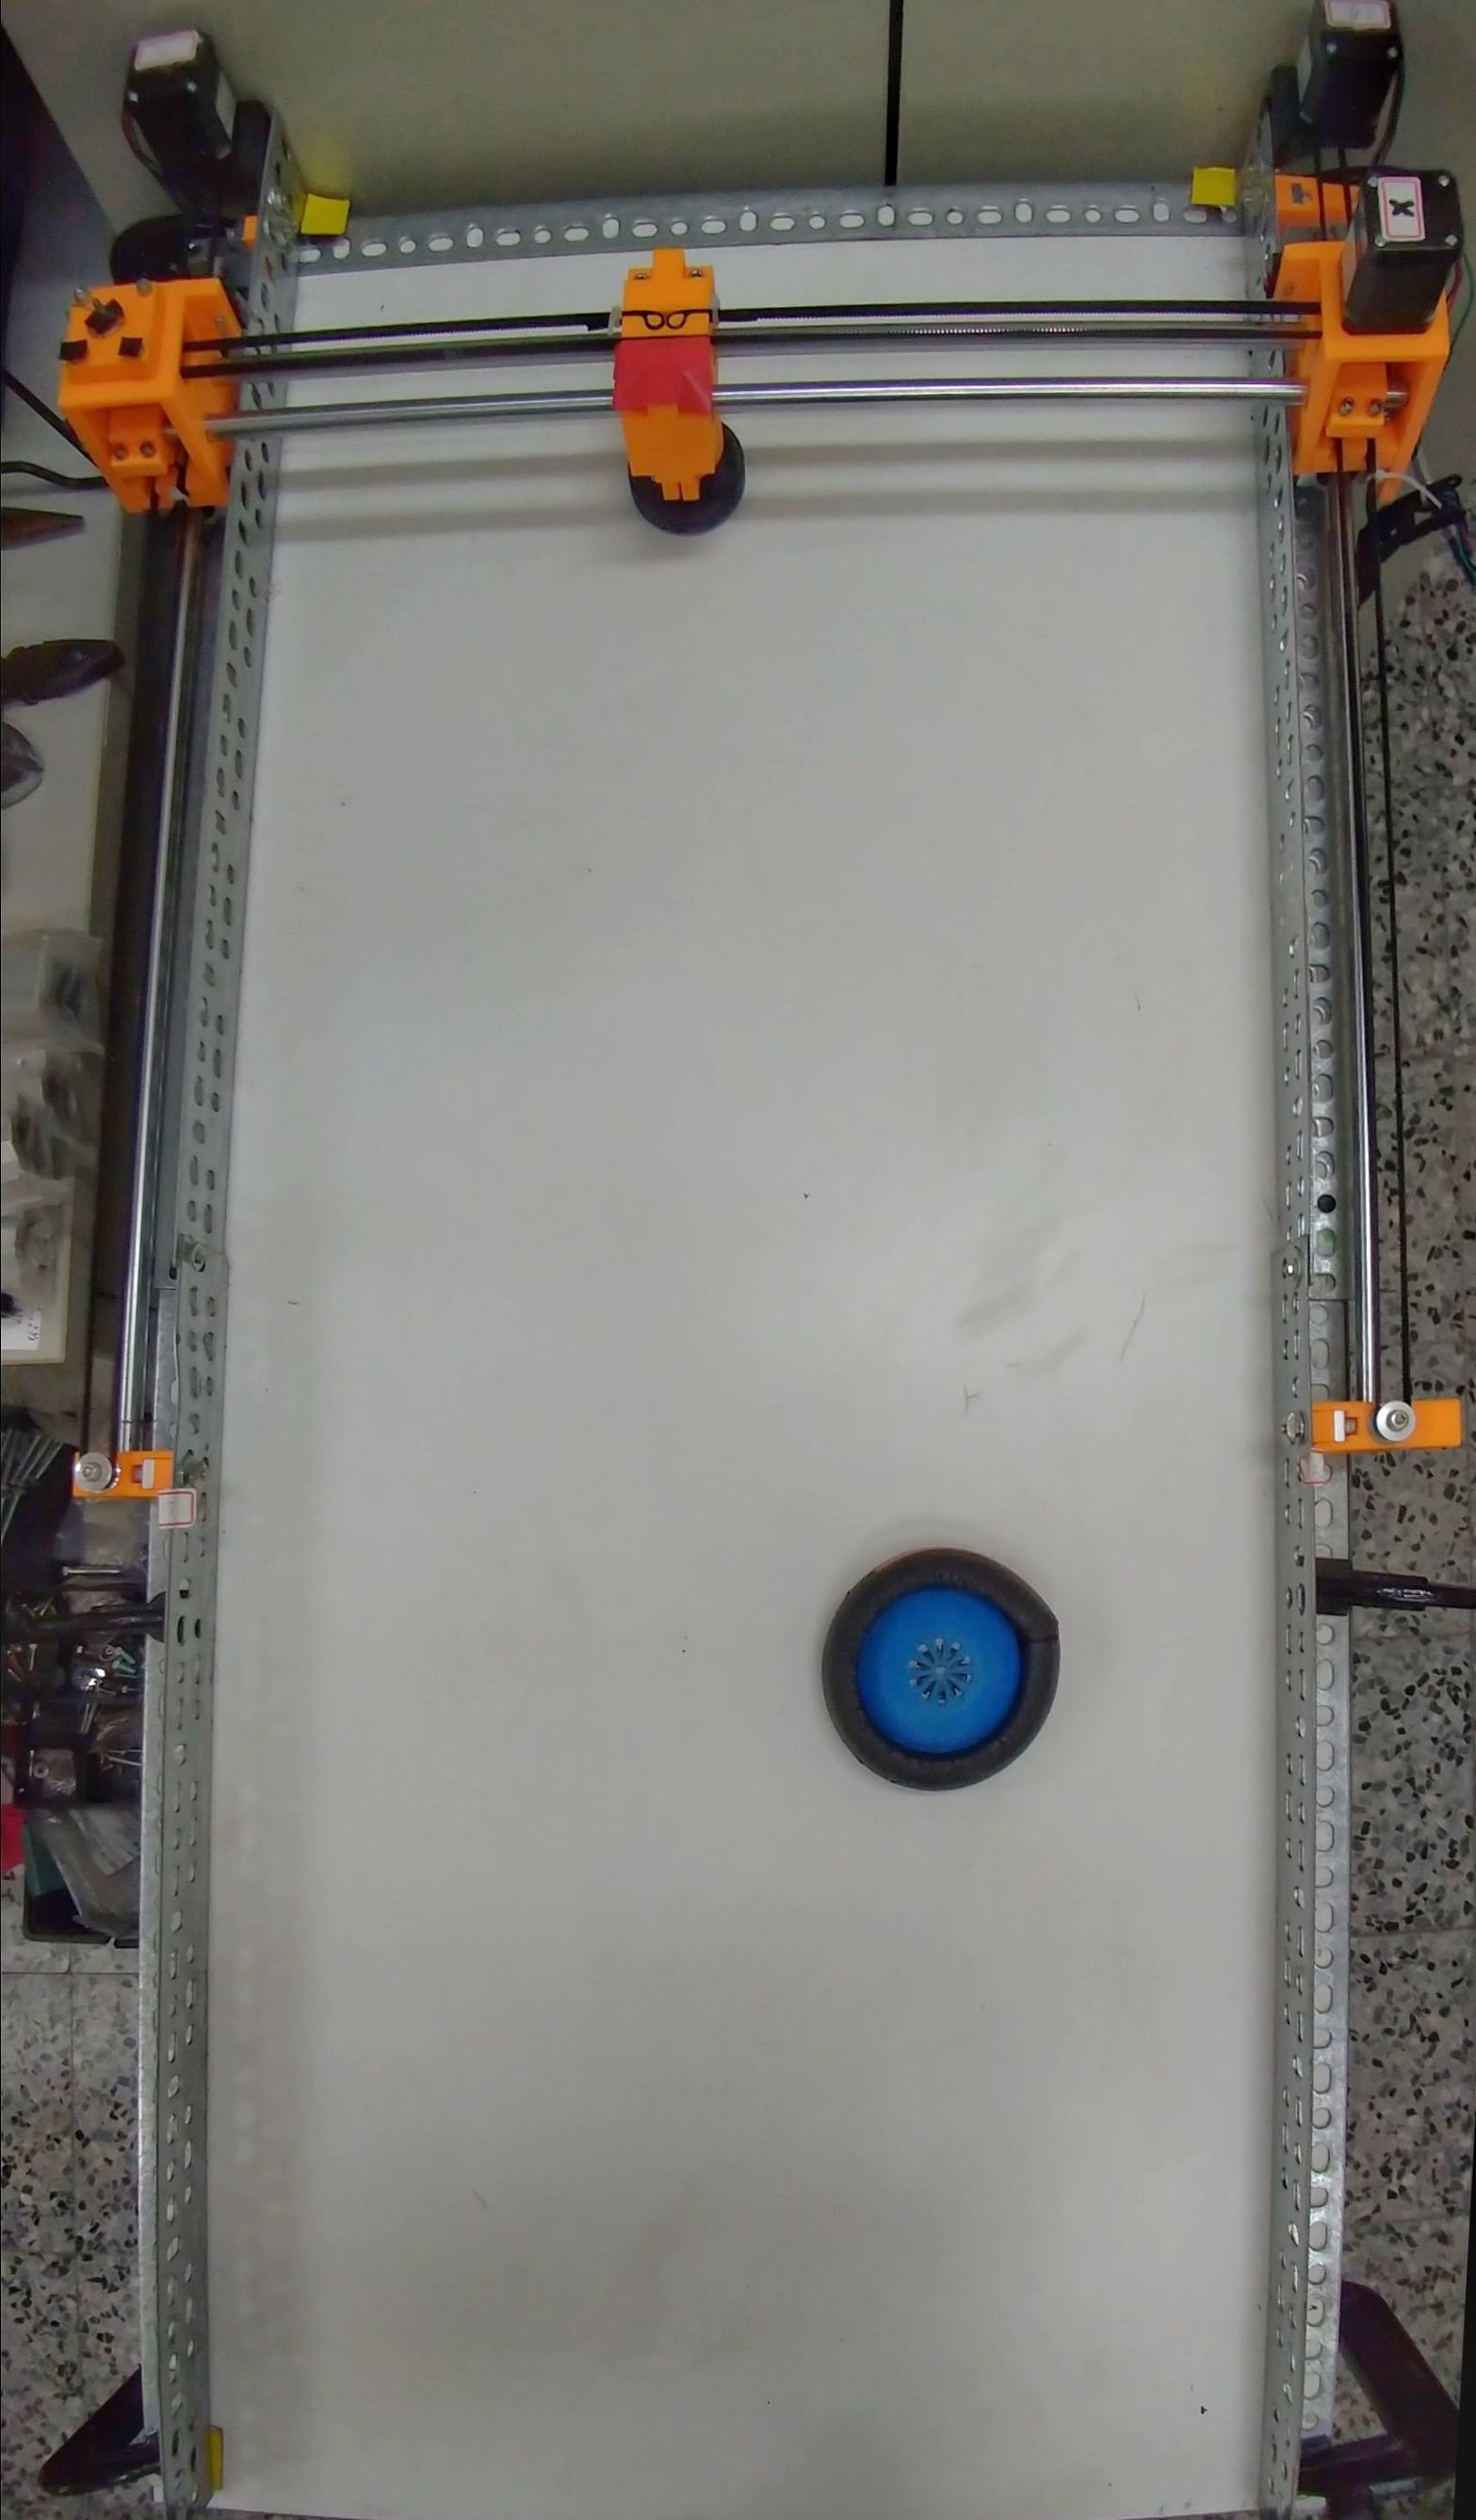
\includegraphics[angle=90,width=10cm]{冰球機}
\caption{\Large 實體的冰球機}\label{fig.冰球機}
\end{center}
\end{figure}
\begin{figure}[hbt!]
\begin{center}
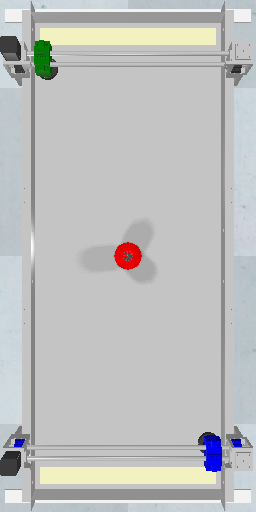
\includegraphics[angle=90,width=10cm]{origin}
\caption{\Large 虛擬環境簡化後的冰球機}\label{fig.模擬冰球機}
\end{center}
\end{figure}
\begin{figure}[hbt!]
\begin{center}
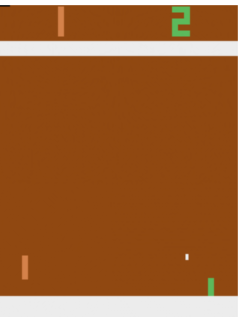
\includegraphics[height=8cm]{pong_gym}
\caption{\Large Gym的Pong game}\label{fig.pong_gym}
\end{center}
\end{figure}


\section{研究目的與方法}
本研究分三大部分,第一運用OpenAI Gym裡內建編譯的ATARI 2600遊戲Pong-v0,來作為訓練環境,加上強化學習的理論,測試不同演算法參數以訓練出最佳化的對打系統,第二將整個簡化後冰球機導入CoppilaSim模擬環境並嘗試進行虛擬訓練,成為優化的對打機電系統。第三則是嘗試透過架設伺服器與虛擬環境結合。\\
 
透過簡化實體冰球機並導入虛擬環境,進行虛擬訓練,使用Gym的Pong當作對應的2D虛擬訓練環境,測試算法和訓練效果,篩選適合的算法與參數。\\

建置CoppilaSim模擬環境,嘗試將2D訓練概念套用到3D環境進行測試,加入電腦視覺與RemoteAPI,電腦視覺抓取球與擊錘的位置,透過RemoteAPI進行遠端控制,在3D環境測試算法可確保後續套用到實體機器上的可行性。\\
 
 再透過架設伺服器與虛擬環境結合:讓虛擬環境的影像透過網伺服器串流影像供使用者遠端進行操控虛擬環境的擊錘進行打球,或是提供多人進行觀看對打影像。
\begin{figure}[hbt!]
\begin{center}
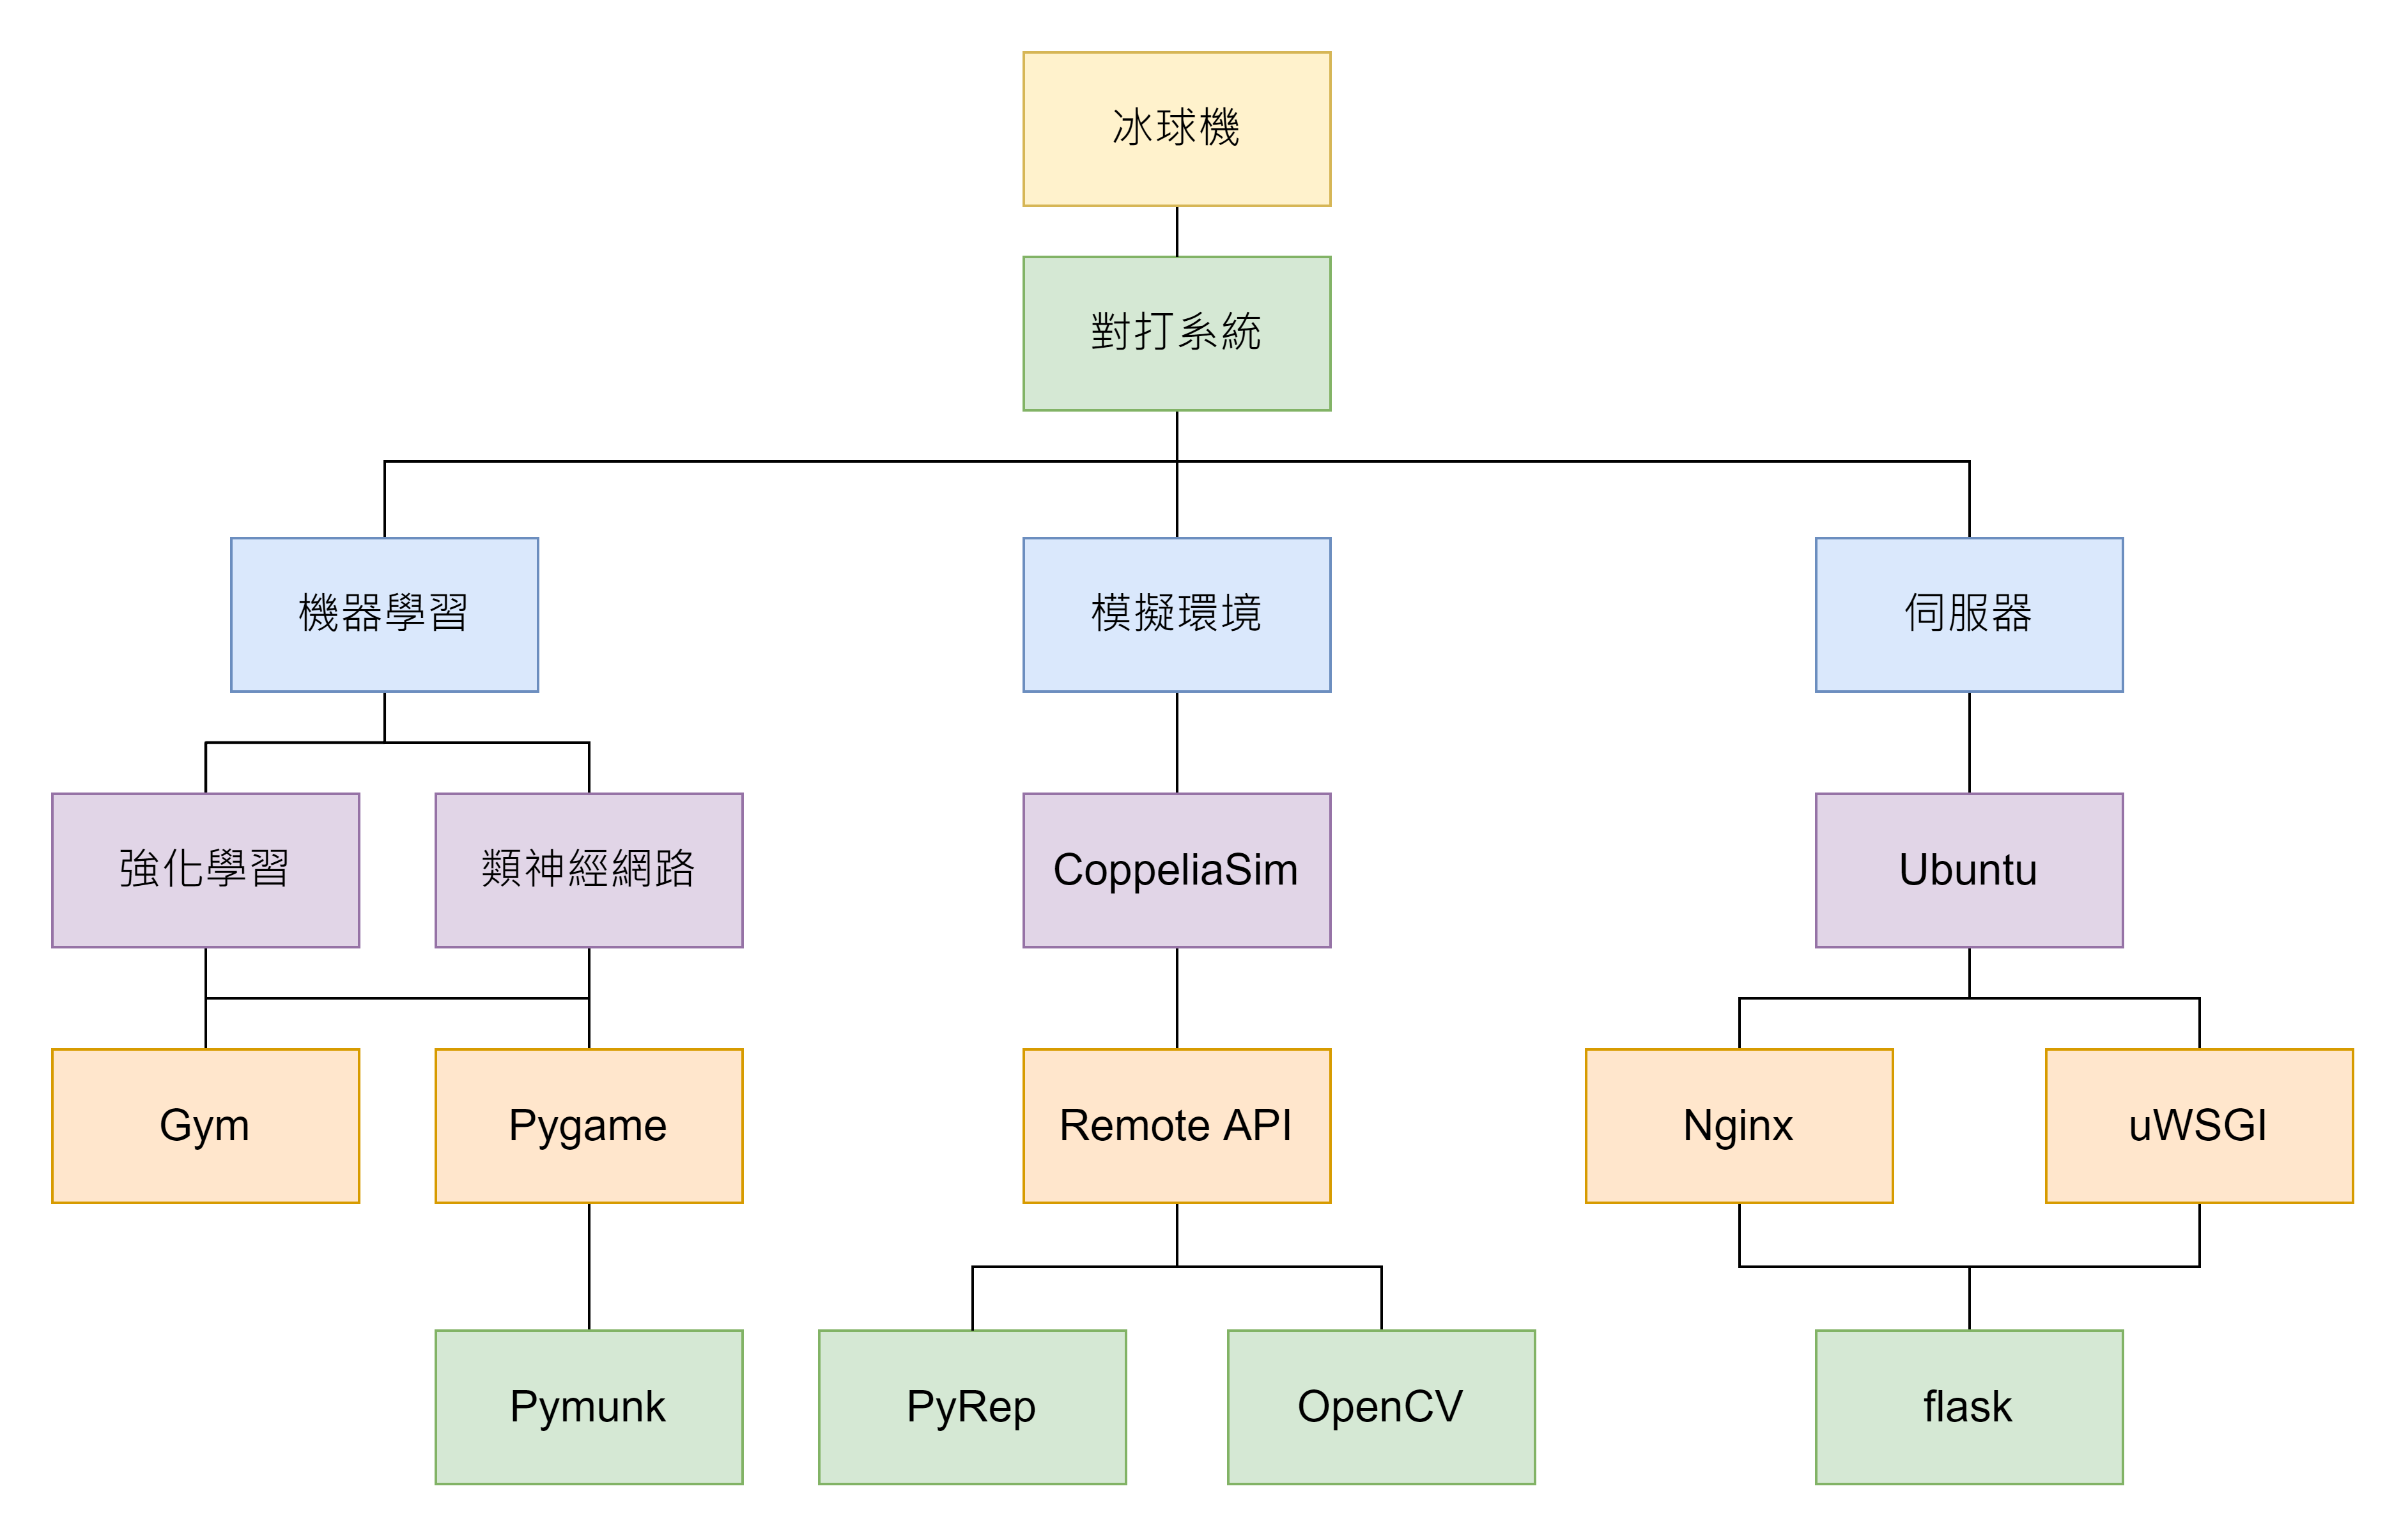
\includegraphics[width=15cm]{研究架構}
\caption{\Large 研究架構 }
\label{研究架構 }
\end{center}
\end{figure}
\section{未來展望}
此專題希望能利用現有完成的機械學習的算法,能發展成虛擬訓練,再將訓練完的機器學習應用到虛擬環境或是實體機電系統,並透過伺服器將影像串流提供玩家網頁介面進行遠端操控,同時提供多人觀看及時的比賽影像,將整個冰球機的控制和使用者間有更完善串聯,機電系統的部分達到最優化控制和虛實整合的應用。
\section{規則說明}
 Pong game 的遊戲規則簡單,透過擊錘將球打入對方球門即得一分,只要其中一方得21分就結束該局。擊錘只能沿單方向來回移動來進行防守和進攻。\\
遊戲規則如下:
\begin{enumerate}
\item 球打入敵方即得一分。
\item 擊錘只單一方向移動。
\item 最快贏得21分者獲勝,並結束該局遊戲。
\end{enumerate}

\renewcommand{\baselinestretch}{0.5} %設定行距
\chapter{實體環境}

\section{3D列印機介紹}

\subsection{FIBR3DEmul}


 採用FIBR3DEmul,他的基層製造技術是將材料加熱後施加壓力噴嘴擠壓出來而定型,一層層的堆疊而形成三維的立體形狀。\\
 
 幾乎所有的基層製造系統一樣,擠製的基礎機器都是採用STL格式的CAD檔,零件的精度是由精度維持的,故輪廓會以較慢的速度製作,而輪廓是由從STL檔的平面和三角形之間提取的交點來做決定,這個方式最突出的優點是在任何想要的座標可以容易的切割。\\

 在成型設備上採用直角座標系統,其工作方式主要是通過完成沿著X、Y、Z軸上的線性運動,驅動單元是以伺服馬達或步進馬達為主,以線性滑軌或同步皮帶搭配齒輪或齒條作為傳動元件所架構起來的機械系統。\\

 原形的強度與填充率有關,強度減弱是孔隙率造成的,而孔洞大小是由填料密度去做選擇。\\

 擠製成型的技術結構中,擠製頭大多藉由切層軟體轉換機械指令GCode來執行點座標的材料塗層路徑,其中提升Z軸升降的穩定性、熔絲擠出量的控制及環境溫度差異變引起的材料熱收縮皆會影響疊層精度的表現,目前都是以手動調整彈簧機構來維持平台角度但此方法無法有效解決平台本身弧形的高低差,而G92是透過安裝於效應器上的現為開關偵測,藉由現為開關的觸發機制,以利於傳回平台與每個Z軸座標點的高度資料,當訊號傳回去時,立即儲存該點位置高度,並採線性補差方式來獲得完整的水平成型面。\\



\chapter{虛擬環境}
%\renewcommand{\baselinestretch}{10.0} %設定行距


\section{CoppeliaSim 場景}
 CoppeliaSim是一套具有整合開發環境的機器人模擬軟體,基於分佈式控制體系架構,可以利用寫入嵌入式腳本、插件、ROS、BlueZero節點、RemoteAPI客戶端或自定義解決方案達成模型控制之效果。\\
\begin{figure}[hbt!]
\center

\includegraphics[width=10cm]{CoppeliaSim}
\caption{\Large CoppeliaSim Logo}
\end{figure}

並且在CoppeliaSim中,控制器可以用C / C ++、Python、Java、Lua、Matlab或Octave進行編寫。\\
\subsection{使用原因}
 本模擬之最終目標是希望可以在虛擬環境中進行3D列印的結果展示,通過虛擬環境中的模擬後,在每次修改零件並更新Gcode後可以直接展示列印的狀況,且在虛擬環境中不會有費用的支出,所以可以用於檢視所列印出之成果後,再進行圖檔修正或設計修改,除此之外CoppeliaSim的虛擬環境更接近真實環境,基於以上原因,所以此專題選擇CoppeliaSim做為模擬的環境。\\
\subsection{RemoteAPI}
 RemoteAPI(Remote Application Programming Interface)是CoppeliaSim API框架的一部分。它允許CoppeliaSim與外部應用程序之間的通訊,是跨平台並支持服務調用和雙向數據流。有兩個不同的版本/框架分別為:Remote API 和The B0-based remote API。\\
\subsection{功能列}
\begin{enumerate}
\item 以下為簡易功能說明:
\begin{figure}[hbt!]
\center
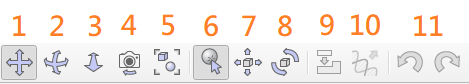
\includegraphics[width=11cm]{toolBar}
\caption{\Large CoppeliaSim 工具列}
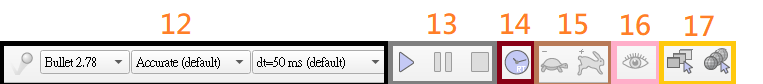
\includegraphics[width=13cm]{toolBar2}
\caption{\Large CoppeliaSim 工具列(續)}
\end{figure}
\begin{table}[hbt!]
\center
\large
\setlength{\tabcolsep}{0.75cm}{
\begin{tabular}{|c|c|c|c|}
\hline  代號 & 功能說明 & 代號 & 功能說明\\
\hline  1 &畫面平移& 10 &複製所有設定\\
\hline  2 &畫面旋轉& 11 &回復/取消回復\\
\hline  3 &畫面縮放&12&模擬設定\\
\hline  4 &畫面視角&13&開始/暫停/停止 模擬\\
\hline  5 &畫面縮放至適當大小&14&即時模擬切換\\
\hline  6 &選取物件&15&模擬速度控制\\
\hline  7 &移動物件&16&線程渲染/視覺化\\
\hline  8 &旋轉物件&17&場景/頁面 選擇\\
\hline  9 &加入/移出 樹狀結構&&\\
\hline
\end{tabular}}
\caption{\Large 功能說明}
\end{table}
\newpage
%\item 模擬執行\\%
\end{enumerate}


\section{FIBR3DEmul printer}
 FIBR3DEmul--是一個適用於3軸或3軸以上的FDM(熔融沉積成型)列印機,進行虛擬列印的開源軟體,在它之中包含了GCodeInterpreter(GCode解析器)、使用CMake生成的simExtFIBR3D.dll\\
 
\subsection{GCodeInterpreter}
\begin{figure}[hbt!]
\begin{center}
\includegraphics[width=14cm]{Gcode}
\caption{\Large GCodeInterpreter 介面功能介紹}\label{GCode}
\end{center}
\end{figure}
\newpage

 \subsection{模擬模型}
 在模擬的模型上,延用了學長之前組建的實體3D列印機,並將其轉為虛擬模型後放入CoppeliaSim,進行組裝、配置後以simExtFIBR3D.dll擴充CoppeliaSim將其與GCodeInterpreter程式進行整合,用以達成使用GCode控制CoppeliaSim中的3D列印機進行模擬列印展示之功能。\\
\begin{figure}[hbt!]
\center
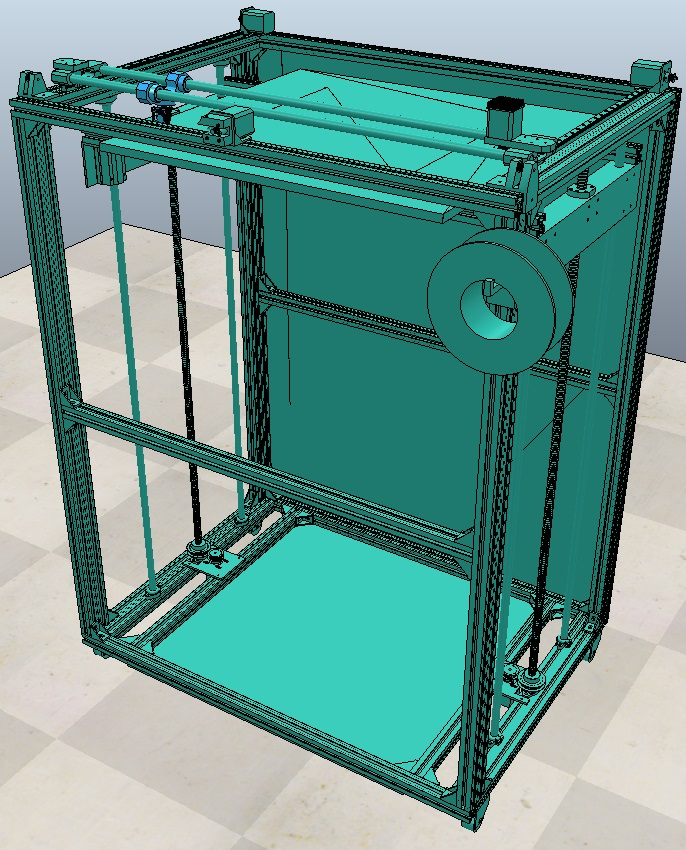
\includegraphics[width=13cm]{組合圖}
\caption{\Large 組合圖}
\label{組合圖}
\end{figure}

\section{虛擬uArm機械手臂}

\section{模擬流程}

\subsection{使用Inventor繪製uArm零件}
 模擬的第一步是先將設計後的uArm零件使用Inventor繪製出來後,再將其轉為Cura程式可接受的STL檔案格式。\\
\begin{figure}[hbt!]
\begin{center}
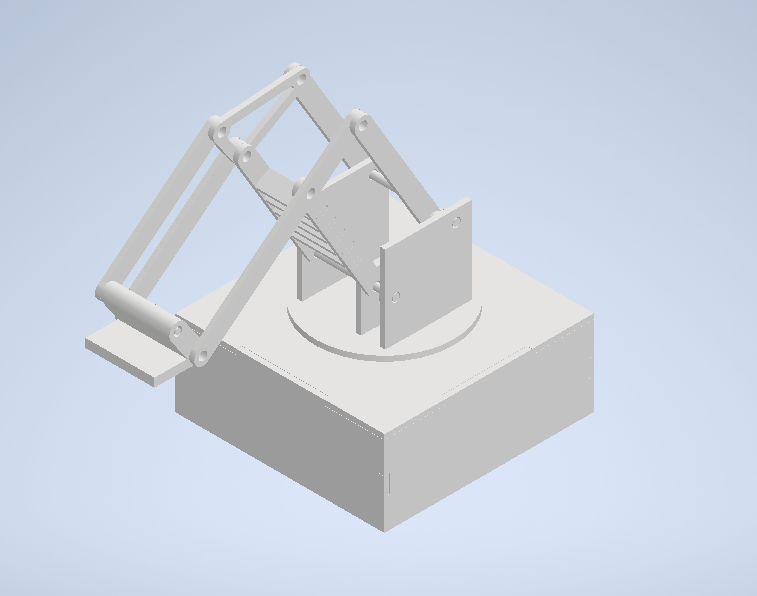
\includegraphics[width=8cm]{Inventor1}
\caption{\Large 使用Inventor繪製零件}\label{Inventor1}
\end{center}
\end{figure}
\subsection{使用Cura轉出G-Code檔}
 第二步將把上一步轉出的STL檔案轉入Cura程式中,可將零件們進行排列或旋轉方向放置到最佳的列印位置,進行切片後,轉出所需的G-Code檔案。\\
\begin{figure}[hbt!]
\begin{center}
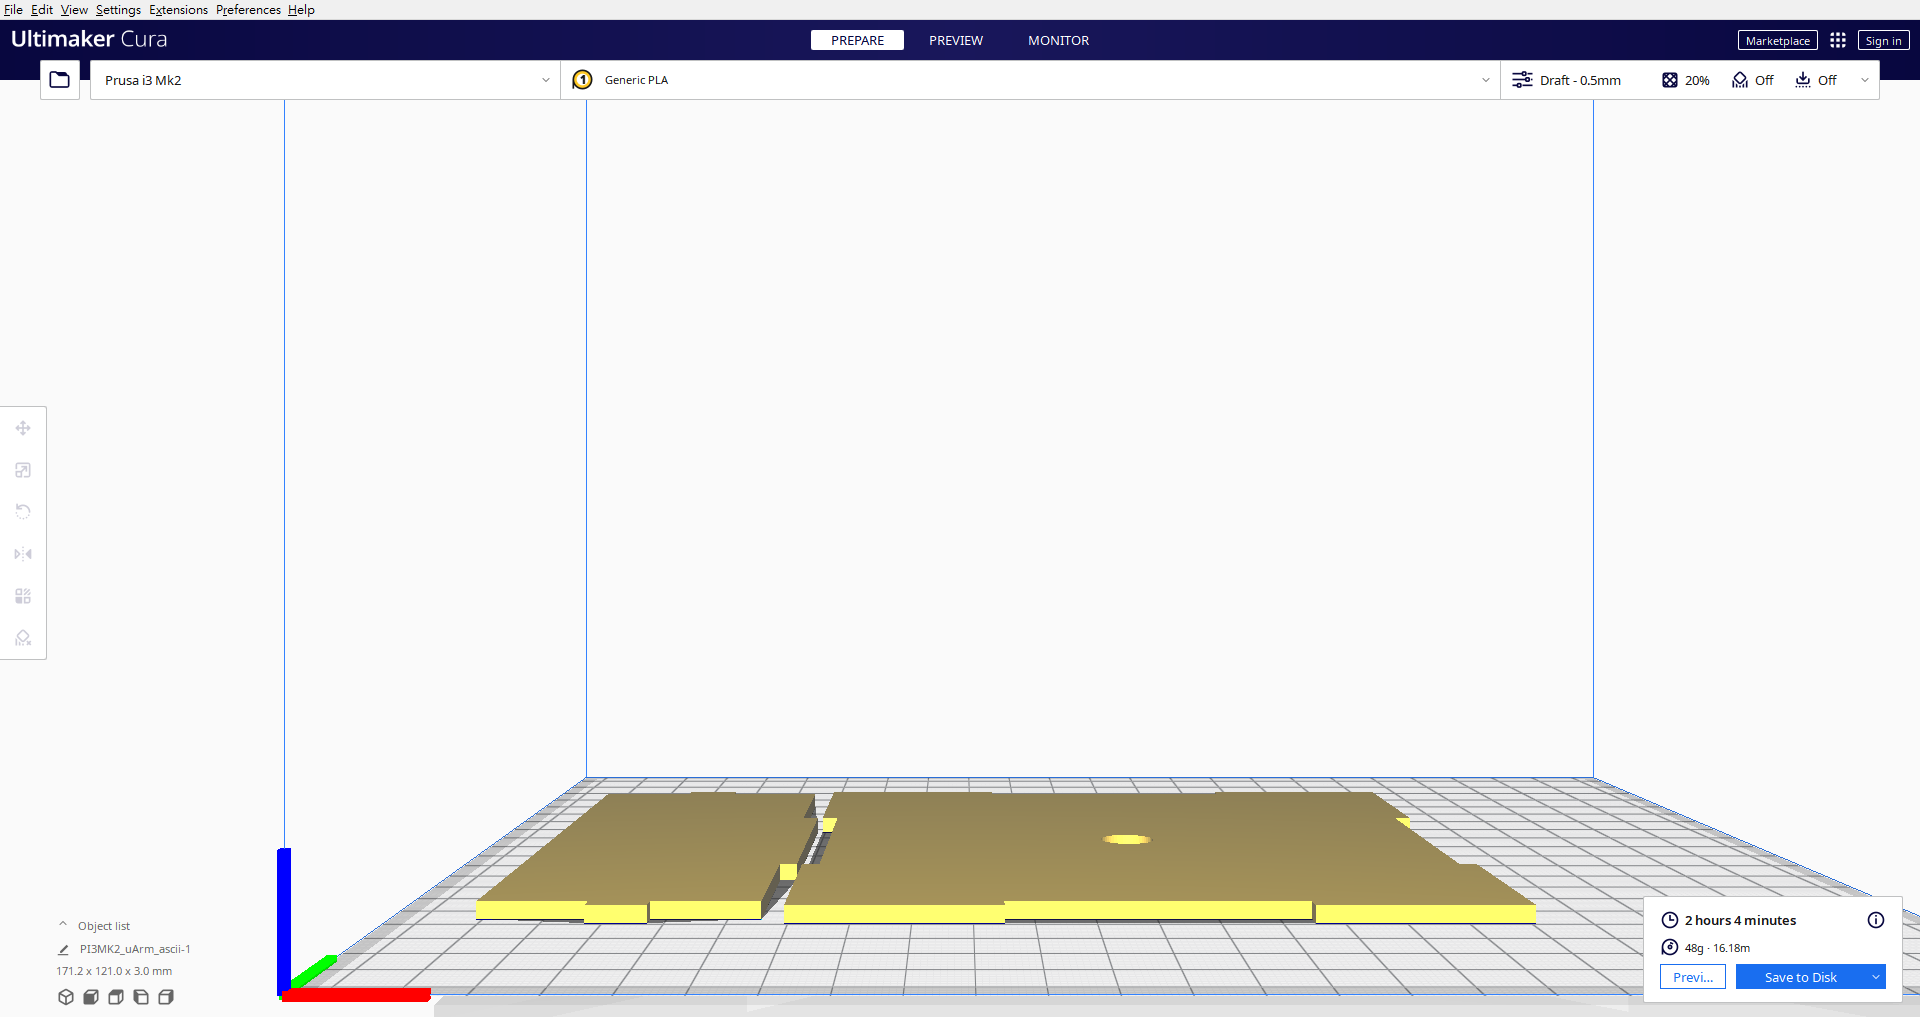
\includegraphics[width=14cm]{Cura}
\caption{\Large 用於轉出 G-Ccode 檔的切片軟體 Cura}\label{Cura}
\end{center}
\end{figure}
\subsection{更改G-Code檔}
 由於此列印模組之Z軸與本專題之3D列印機恰好相反,因此需修改有關的Z軸代碼後的數值為負值,還有一處需要修改,那就是擠出率的代碼,列印模組中擠出率代碼為A,但從Cura中轉出的G-Code中擠出率代碼為E,所以需將G-Code中的代碼E更改為A。
\begin{figure}[hbt!]
\begin{center}
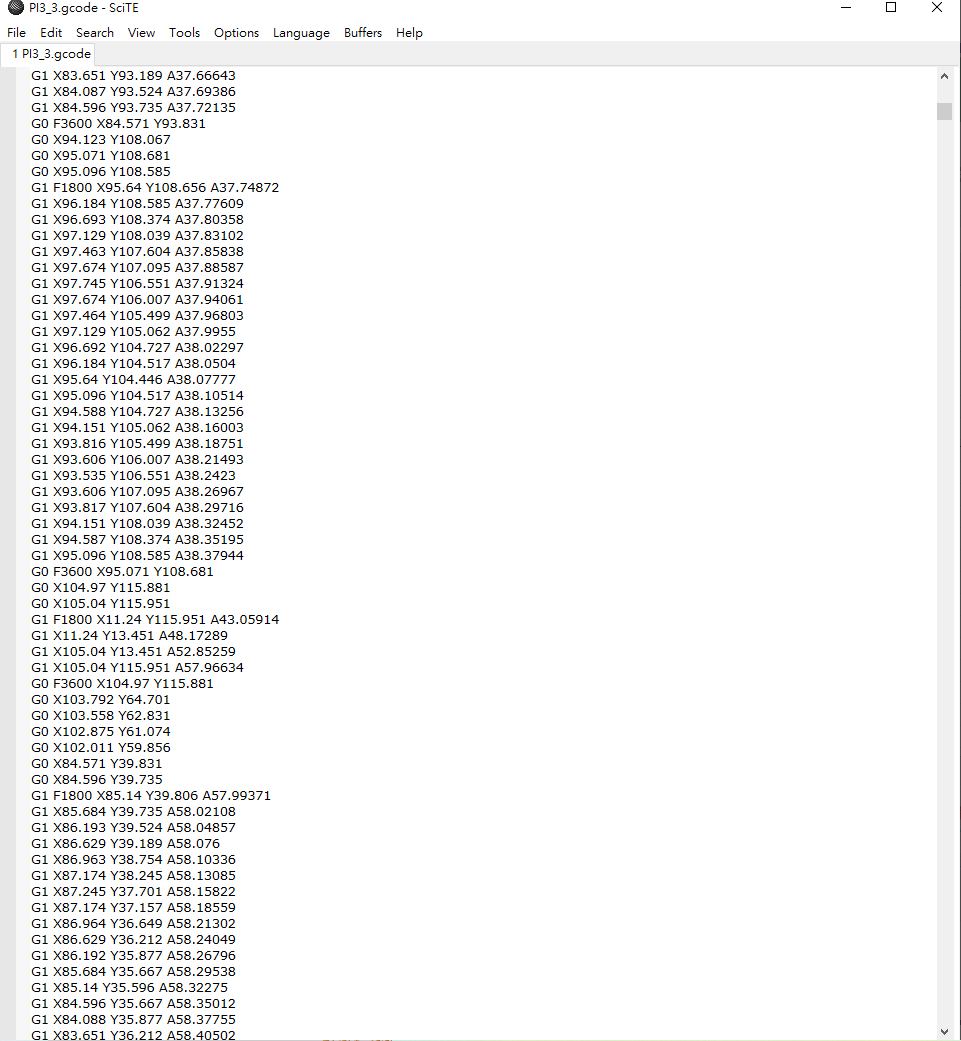
\includegraphics[width=14cm]{修改GCODE}
\caption{\Large 修改G-Code部分代碼}\label{修改GCODE}
\end{center}
\end{figure}
\\subsection{將G-Code轉入GCodeInterpreter}
 第四步將修改好的G-Code檔案轉入GCodeInterpreter,按下連接鍵與CoppeliaSim連接後,進行模擬。\\
\begin{figure}[hbt!]
\begin{center}
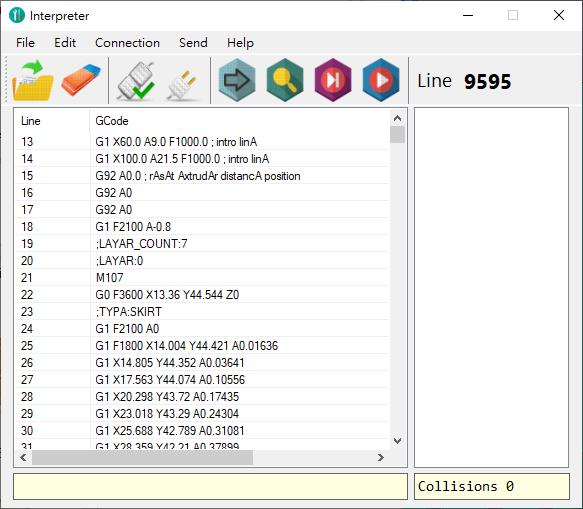
\includegraphics[width=14cm]{GCodeInterpreter}
\caption{\Large 模擬中的GCodeInterpreter畫面}\label{GCodeInterpreter}
\end{center}
\end{figure}
\\subsection{uArm零件模擬列印結果}
 在CoppeliaSim模擬設定視窗中可以調整擠出材料的大小以及形狀(圓球或方塊),與GCodeInterpreter連接後,當GCodeInterpreter按下運行鍵後,開始列印模擬,在CoppeliaSim中也可以進行模擬列印整體速度調整,更加省時,下圖為模擬結果。\\
\begin{figure}[hbt!]
\begin{center}
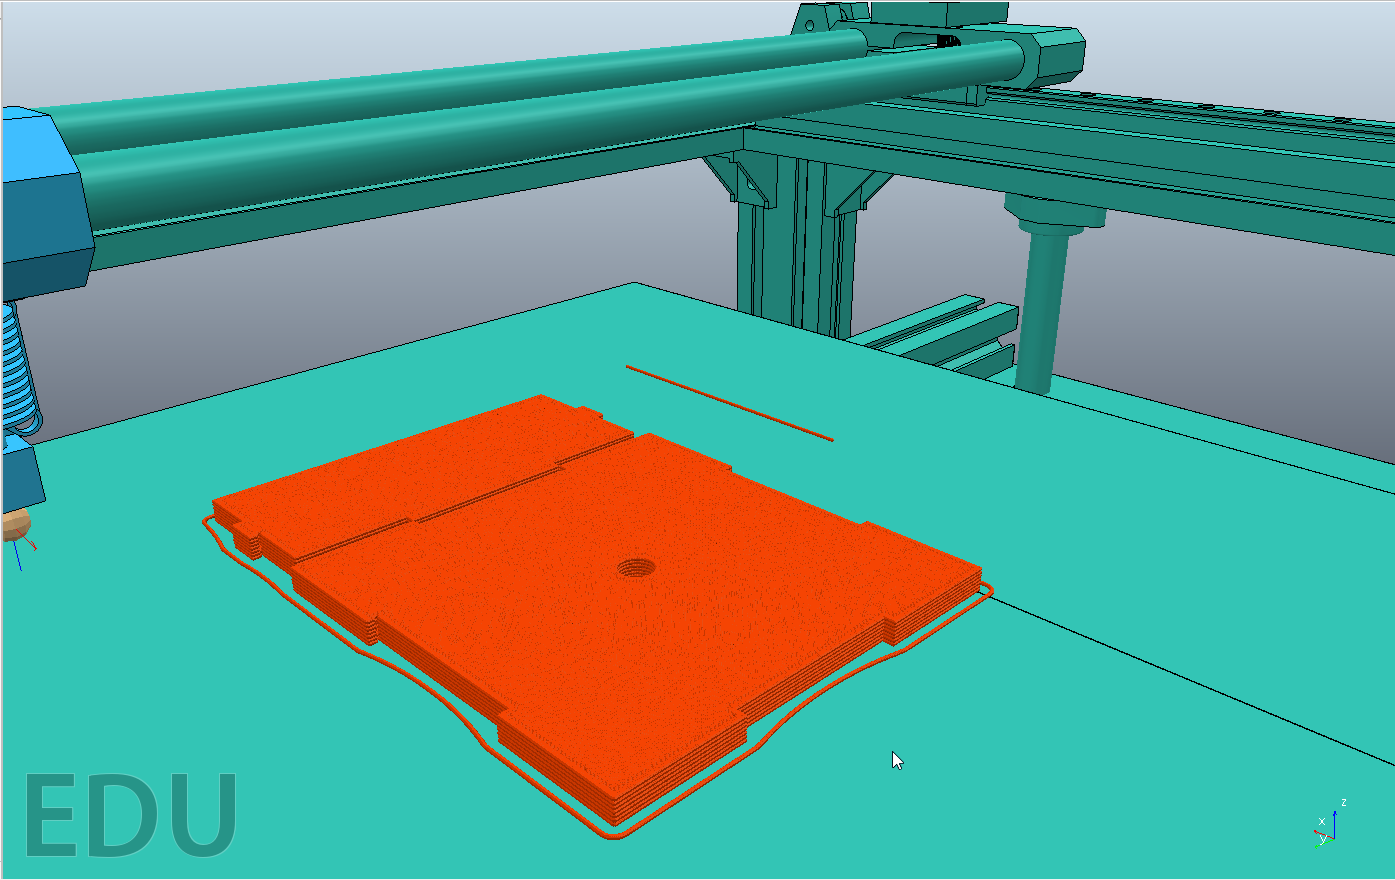
\includegraphics[width=14cm]{simulation}
\caption{\Large 模擬列印結果}\label{simulation}
\end{center}
\end{figure}

\begin{figure}[hbt!]
\begin{center}
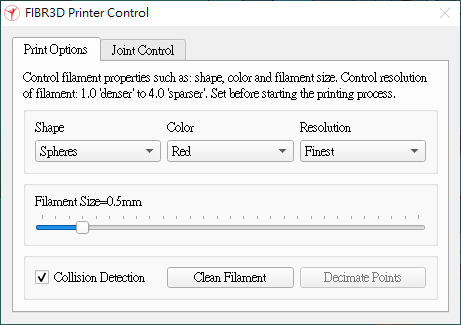
\includegraphics[width=12cm]{UIP}
\caption{\Large 列印選項控制 UI介面}\label{UIP}
\end{center}
\end{figure}

\subsection{在CoppeliaSim匯入uArm零件進行模擬}
 將uArm的STL檔匯入CoppeliaSim中將零件進行拆解並簡化,接著是各軸的組配,最後搭配CoppeliaSim的UI進行三個馬達軸的控制。\\
 
\subsection{簡化模型}
 所謂的簡化係指將uArm STL檔轉進CoppeliaSim拆解後,進入Toggle shape edit mode(三角形編輯模式)針對各零件的三角網格進行選擇後,從複雜形狀的零件簡化提取出方塊、圓柱或圓球等等的簡單形狀,用於模擬運算,外觀可套上原零件保持原樣,另一方式為使用add選單中的Convex decomposition of selection(凸分解),Convex Hull(凸包)可以理解在高維空間中有一群散佈各處的點,「凸包」是包覆這群點的所有外殼當中,表面積暨容積最小的一個外殼,而最小的外殼一定是凸的。而凸分解就是將零件依據三角網格的頂點分解成數個凸包再進行組合,在運算效率上來說使用Toggle shape edit mode(三角形編輯模式)方式可獲得較好的效果。\\
 
\begin{figure}[hbt!]
\begin{center}
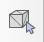
\includegraphics[width=2cm]{TSEM}
\caption{\Large Toggle shape edit mode(三角形編輯模式)}\label{TSEM}
\end{center}
\end{figure}

\begin{figure}[hbt!]
\begin{center}
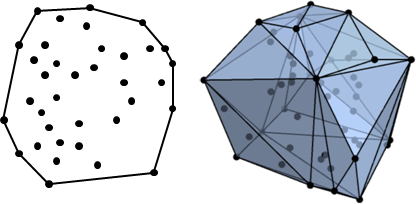
\includegraphics[width=10cm]{ConvexHull1}
\caption{\Large Convex Hull(凸包)}\label{ConvexHull1}
\end{center}
\end{figure}

\subsection{模擬}
 一開始使用官方圖檔進行模擬,花費許多組配時間在簡化零件之上,所以決定使用自行繪製的簡化圖檔進行模擬,簡化圖檔保留了主要的零件,設計後的零件大部分為利於列印的薄板件。\\
\begin{figure}[hbt!]
\begin{center}
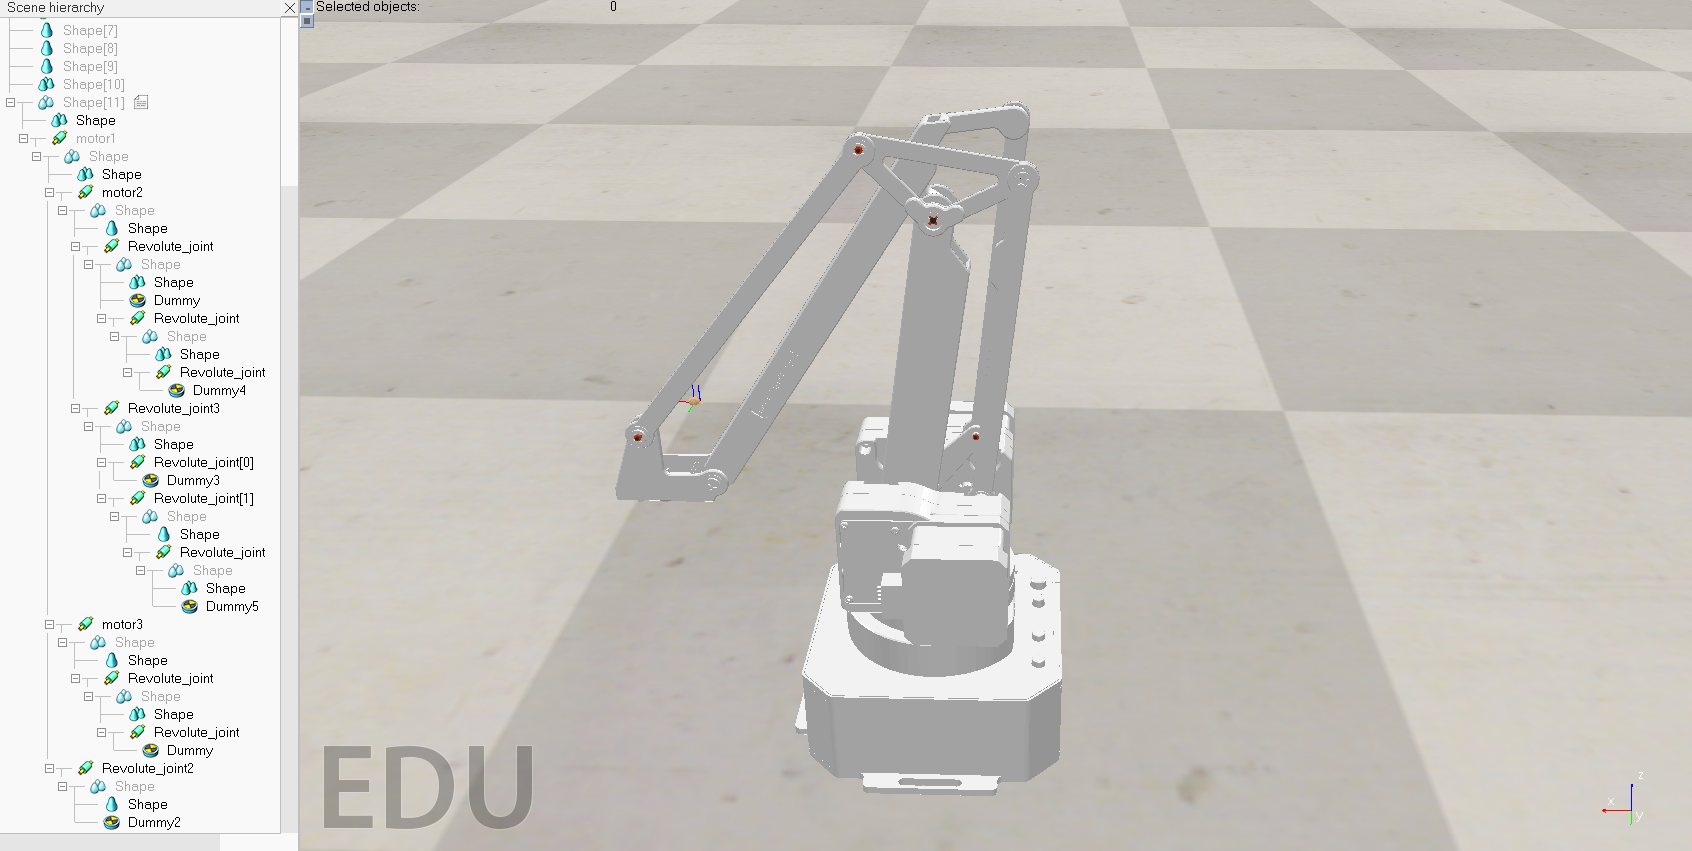
\includegraphics[width=14cm]{uArm01}
\caption{\Large 原版的uArm手臂模擬}\label{uArm01}
\end{center}
\end{figure}
\begin{figure}[hbt!]
\begin{center}
\includegraphics[width=14cm]{uArm02}
\caption{\Large 設計過後的uArm手臂模擬}\label{uArm02}
\end{center}
\end{figure}
\begin{figure}[hbt!]
\begin{center}
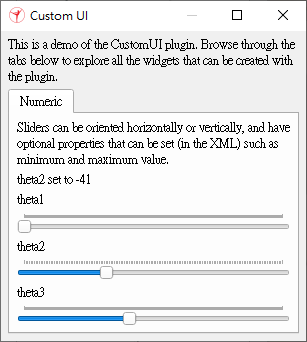
\includegraphics[width=12cm]{UI}
\caption{\Large 用於控制3個馬達軸的UI介面}\label{UI}
\end{center}
\end{figure}
\newpage


\chapter{座標轉換}
\subsection{3D座標提取}

座標轉換是為了將複雜積分或傅立葉級數轉換為簡單質關的公式,讓他變成最基本的三角形或四面體網格去計算,再將所有網格的值相加,得到體積極慣性矩後求得質心。\\

\begin{itemize}
%=----------Sigmoid      Function----------=%
\item 網格及法線的形成(圖.\ref{三角網格法線方向}):\\
STL文件表示的表面是封閉並連接的三角形網格,其中每條邊都是兩個三角形的一部分,並且不相交。對於一個三角形,可以通過頂點的順序和右手定則來決定,如果公共邊有不同的方向,就可以證明兩個三角形的法線是一致的。\\
\begin{figure}[hbt!]
\begin{center}
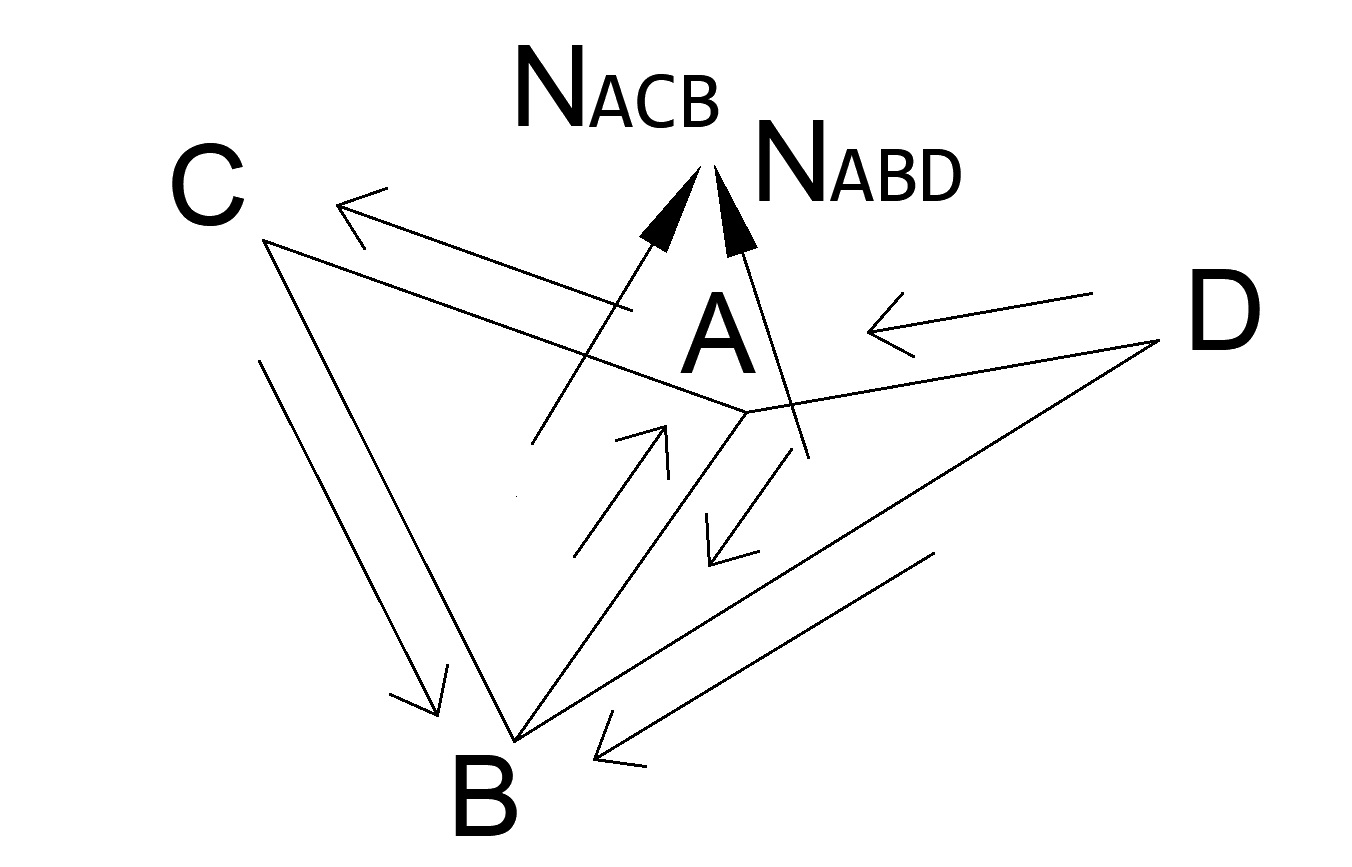
\includegraphics[width=16cm]{三角網格法線方向}
\caption{\Large 三角網格法線方向}\label{三角網格法線方向}
\end{center}
\end{figure}
\\
%=----------Softmax Function----------=%
\item 四面體體積(圖.\ref{3D體積的計算}):\\
在3D情況下,計算的基本單元為四面體,將原點與三角形的各個頂點連接形成一個四面體。三角形ACB具有法線NACB,由於原點 O 位於 NACB 的對面,因此這個四面體的值是正的,體積也可以由內積 OA $\cdot$ NACB 判斷。四面體體積為:\\
$$ V'_t = \frac{1}{6}(-x_3i y_2i z_1i + x_2i y_3i z_1i + x_3i y_1i z_2i - x_1i y_3i z_2i - x_2i y_1i z_3i + x_1i y_2i z_3i) $$
$$ V'_total= \sum_{i}V'_i$$

\begin{figure}[hbt!]
\begin{center}
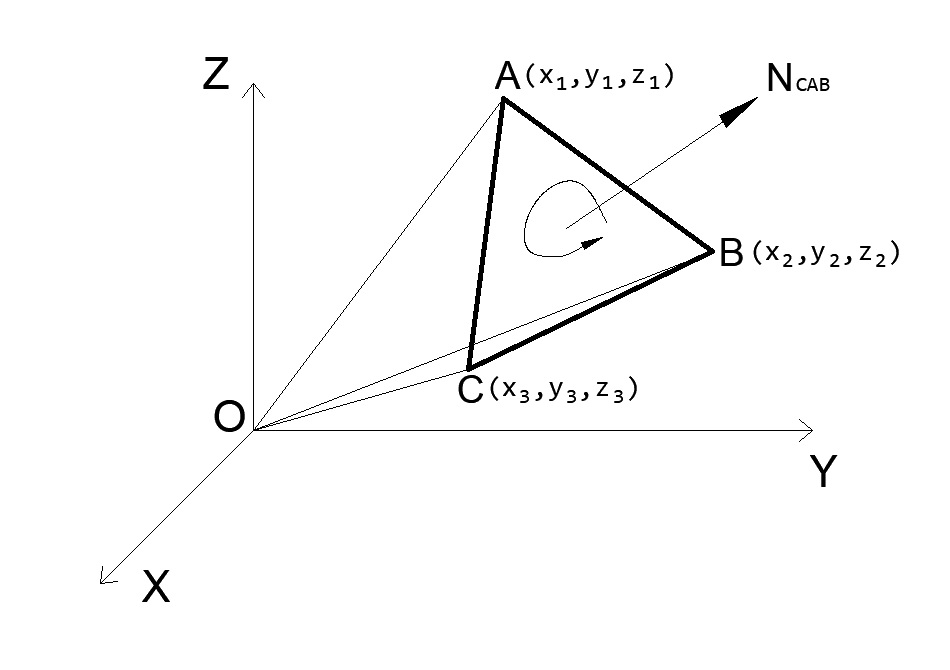
\includegraphics[width=16cm]{3D體積的計算}
\caption{\Large 3D體積的計算}\label{3D體積的計算}
\end{center}
\end{figure}
%=----------Relu Function----------=%
\item 空間裡的體積:\\
計算的特徵可以寫為帶有作標總和的基礎特徵形狀,並且可以以顯式倒出基本形狀,雖然這是一個很大的約束,但是在內部空間上具有積分形式都可以使用。\\
 p, q, r 為矩的階,中心矩可以從下列求解:\\

$$M_{pqr} = \iiint x^{p} y^{q} z^{r} \rho (x,y,z) \,dx\,dy\,dz$$
其中 $\rho (x,y,z)$ 是基礎形狀i的指示函數:\\
\begin{equation}
\label{eq6}
\rho (x,y,z) = \left\{
\begin{aligned}
1 & , & if (x,y,z) is inside the mesh\\
0 & , &              otherwise
\end{aligned}
\right.
\end{equation}
$S_i$ 是形狀i做有標記座標的體積的符號函數,積分可以重寫為每個基本形狀的積分之和:\\
$$M_pqr = \sum_{i} S_i \iiint x^{p} y^{q} z^{r} \rho_i (x,y,z) \,dx\,dy\,dz$$

由於物體內部的空間可以使用傅里葉變換,也能通過將積分分解為每個基本形狀的積分來計算。二維的傅里葉轉換或 3D 網格模型由傅里葉變換定義其指示函數:\\

$$ \Theta (u,v,w) = \iiint e^{-i (xu+yv+zw)} \rho (x,y,z) \,dx\,dy\,dz $$

\item 產生矩陣:\\
主軸是通過計算矩陣 S 的特徵向量獲得的,也稱為主成分分析 (PCA)。 將最大特徵值對應的特徵向量作為第一主軸。 第二個特徵值對應的下一個特徵向量是第二個主軸,以此類推。我們進一步確保三階矩 M300 和 M030 變換後是正的,為了使最終結果是唯一的。\\

我們通過 3D 模型的二階矩構造一個 3x3 矩陣:

\[ 
S=\begin{bmatrix} 
M_{200} & M_{110} & M_{101} \\
M_{110} & M_{020} & M_{011} \\
M_{101} & M_{011} & M_{022} 
\end{bmatrix}
\]

\item 總結:\\
要使用pySTL將STL檔在轉入虛擬環境時,坐標軸會產生偏差,需要用到的體積和慣性矩去轉換質心,利用質點繞了座標軸的概念矯正零件的偏差,即可調整物體的角度、移動與比例縮放:\\

$M_{000}$數字符號由左至右分別代表著X、Y、Z,而數字大小則代表冪次數。


體積:$M_{000} = \frac{1}{6}(-x_3 y_2 z_1 + x_2 y_3 z_1 + x_3 y_1 z_2 - x_1 y_3 z_2 - x_2 y_1 z_3 + x_1 y_2 z_3) $\\

對x的一次矩:$M_{100} = \frac{1}{4}(x_1 + x_2 + x_3) M_{000} $\\

對x的二次矩:$M_{200} = \frac{1}{10}(x_1^{2} + x_2^{2} + x_3^{2} + x_1 x_2 + x_2 x_3 + x_1 x_3 ) M_{000} $\\

質點x軸位置:$\frac{M_{100}}{M_{000}} = (\frac{1}{4}(x_1 + x_2 + x_3)) $\\

質點y軸位置:$\frac{M_{010}}{M_{000}} = (\frac{1}{4}(y_1 + y_2 + y_3)) $\\

質點x軸位置:$\frac{M_{001}}{M_{000}} = (\frac{1}{4}(z_1 + z_2 + z_3)) $\\


\end{itemize}
\chapter{pystl}
 pystl是處理stl檔案的python開源程式,無須打開CAD軟體即可編輯操作stl檔案,可以輕易使物體移動、轉動與縮放的動作。目前可以把輸入的ASCLL 或 binary STL檔案全部輸出成ASCLL STL。\\
 

\section{pySTL 功能}
\begin{itemize}
\item 打開text.stl檔案
\begin{lstlisting}[caption=\Large 輸入檔案]
import pySTL
model = pySTL.STLmodel('text.stl')

\end{lstlisting}
 
\item 物體向x軸移動10單位
 \begin{lstlisting}[caption=\Large 移動]
import numpy
movement = numpy.array([10, 0, 0])
model.translate(movement)

\end{lstlisting}

\item 物體質心移動到座標原點
 \begin{lstlisting}[caption=\Large 移動]
model.translate(-c)

\end{lstlisting}

\item 物體向X軸轉90度(角度是徑度)
 \begin{lstlisting}[caption=\Large 轉動]
R= pySTL.rotationAboutX(-3.14149/2)
model.rotate(R)

\end{lstlisting}

\item 物體縮小10%
 \begin{lstlisting}[caption=\Large 縮放]
scale = 0.1
model.scale(scale)

\end{lstlisting}


\item 質心顯示
 \begin{lstlisting}[caption=\Large 數值]
c = model.get_centroid()
print(c)

\end{lstlisting}

\item 體積顯示
 \begin{lstlisting}[caption=\Large 數值]
v = model.get_volume()
print(v)

\end{lstlisting}

\item 產生newText.stl檔案
\end{itemize}
 \begin{lstlisting}[caption=\Large 產生新stl檔案]
model.write_text_stl('newText.stl')
\end{lstlisting}

\section{為何要使用pySTL?}

由於預設場景裡CAD檔案與.STL的座標系是不相同,且.stl(mm)與coppeliasim(m) 的單位也不相同,所以當人們在不同軟體間操作,若是沒有注意到各個檔案的關係,會發生(如:圖5.1)物體方向錯誤或者尺寸錯誤,則必須要打開CAD軟體,使用軟體的移動、旋轉、縮放等工具把問題修正再轉成stl格式放進Coppeliasim場景,這一來一往所花費的時間是耗時的。\\

\begin{figure}[hbt!]
\begin{center}
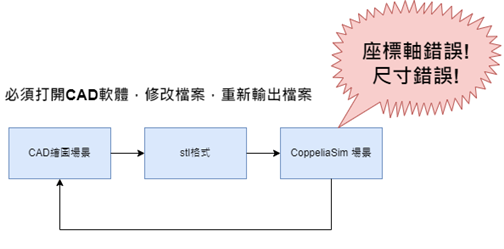
\includegraphics[scale=0.8]{正常轉檔流程}
\caption{\Large 正常轉檔流程}\label{正常轉檔流程}
\end{center}
\end{figure}

當檔案錯誤時,無須打開CAD軟體,只要編輯器啟動pySTL 代碼,輸入想要修改的參數按下執行,即可產生正確且最新版本的stl檔案,有了這項工具,即使電腦裡沒有繪圖軟體,也能立刻修改出正確的檔案,這將會是簡單又省時的操作來完成目標。(如:圖5.2)\\

\begin{figure}[hbt!]
\begin{center}
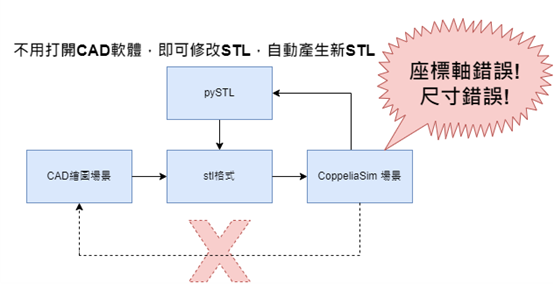
\includegraphics[scale=0.8]{pystl轉檔流程}
\caption{\Large pystl轉檔流程}\label{pystl轉檔流程}
\end{center}
\end{figure}

\section{如何使用pySTL?}
因為pySTL是一個開源套件,所以我們先在github 裡git clone pySTL整個資料夾下載出來。(如:圖5.3)\\

\begin{figure}[hbt!]
\begin{center}

\includegraphics[scale=0.8]{clone pySTL}
\caption{\Large clone pySTL}\label{clone pySTL}
\end{center}
\end{figure}

這裡我們先當作檔案已經排除錯誤可以直接使用,因為資料裡的pySTL.py與sample.py有多處地方是錯誤的需要去解決,我們將詳細的解決步驟放到第8章節的問題討論裡。\\

\section{ pySTL操作設定}
首先打開sample.py檔案,輸入想要操作的名稱的STL檔。\\

 \begin{lstlisting}[caption=\Large 輸入名稱]
import pySTL
from numpy import array

#Load a model from a file.
model = pySTL.STLmodel('uArm_binary.stl')

\end{lstlisting}

在這裡我們選擇的檔案是uArm\_binary.stl檔案,並且可以先使用print,使我們可以先取得原本stl檔案的體積與質心數值。 \\

 \begin{lstlisting}[caption=\Large 數值]
v = model.get_volume()
print(v)

\end{lstlisting}


\begin{figure}[hbt!]
\begin{center}
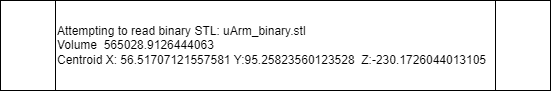
\includegraphics[scale=0.8]{ 體積與質心數值顯示}
\caption{\Large 體積與質心數值顯示}\label{ 體積與質心數值顯示}
\end{center}
\end{figure}

我們輸入pySTL.rotationAboutX(-3.14159/2),使物體能夠向x軸轉動90度,這裡需要注意的點是,角度的單位是徑度。\\

 \begin{lstlisting}[caption=\Large 向X軸轉90度]
#Rotate the model 90 degrees about the X-axis
R2 = pySTL.rotationAboutX(-3.14159/2)

model.rotate(R2)

c = model.get_centroid()
print ("Centroid1 " +  "X: " + str(c[0]) + " Y:" + str(c[1]) + "  Z:" + str(c[2]))

\end{lstlisting}

因為stl檔案的單位mm,但是coppeliasim模擬的場景的單位是m,所以我們必須使用scale=0.001,使物體縮小1000倍在使用model.write\_text\_stl來產生檔案。(如圖:圖5.3)\\

 \begin{lstlisting}[caption=\Large 縮小1000倍]
#Scale the model down by 1000%
scale = 0.001
model.scale(scale)

c = model.get_centroid()
print ("Centroid2 " +  "X: " + str(c[0]) + " Y:" + str(c[1]) + "  Z:" + str(c[2]))
model.write_text_stl('uArm_scale_down_0.001.stl')

\end{lstlisting}

最後我們把生成好的uArm\_scale\_down\_0.001stl放進coppeliasim場景裡面(圖5.4)我們可以發現uArm手臂的尺寸與方向都是正確的,無須再調整。\\

\begin{figure}[hbt!]
\begin{center}
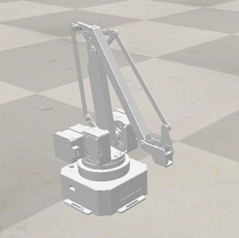
\includegraphics[scale=0.8]{uArm scale down coppeliasim}
\caption{\Large uArm scale down coppeliasim}\label{uArm scale down coppeliasim}
\end{center}
\end{figure}

\section{程式流程}

首先我們執行sample.py的啟動檔,導入pySTL模組,即可讀取STL檔案,得知物體體積與質心數值後,輸入想要的物體位置與比例縮放,來達成最終理想的STL檔案。(圖:5.5)\\

\begin{figure}[hbt!]
\begin{center}
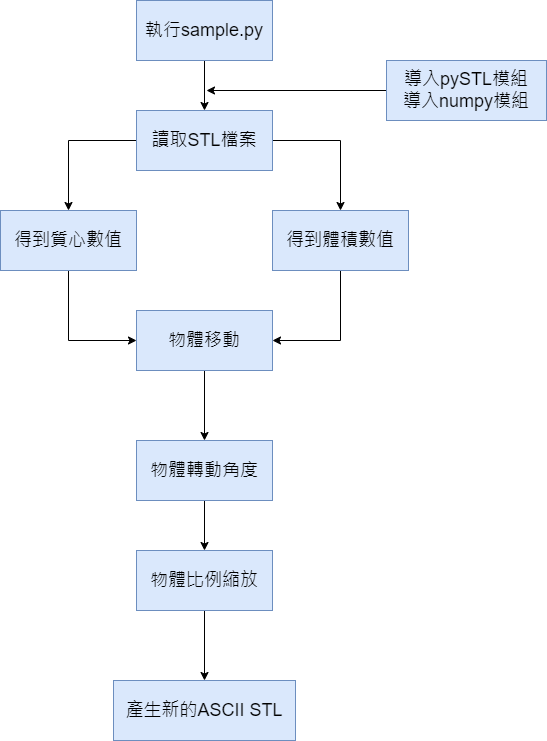
\includegraphics[scale=0.8]{sample.py程式流程}
\caption{\Large sample.py程式流程}\label{sample.py程式流程}
\end{center}
\end{figure}

\subsection{pySTL.py程式流程} 
(圖:5.6)我們讀取STL會先判斷各個種類的STL檔案,分別使用不同的方法去讀取檔案,當可以成功讀取檔案時,我們即可以使用ASCII的規格來寫入進去(solid	表面對法線	三維三角形頂點),即可產生ASCII STL檔案。\\

    我們使用每個三角形的頂點與原點形成一個四面體,計算每個模型體積用於得到三維形狀的質心(使用第6章的理論來求解),即可得用於物體的移動、轉動與縮放。\\

\begin{figure}[hbt!]
\begin{center}
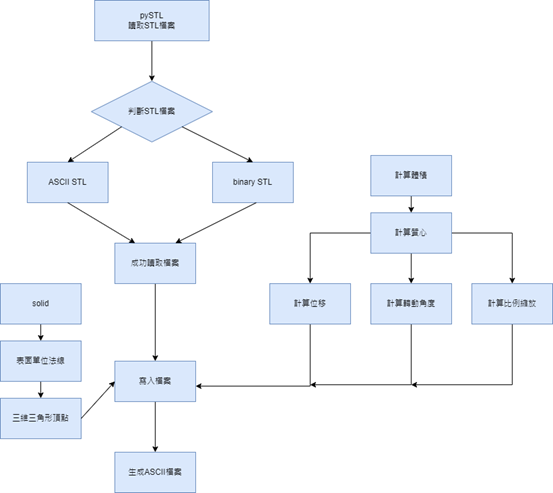
\includegraphics[scale=0.8]{pySTL.py程式流程}
\caption{\Large pySTL.py程式流程}\label{pySTL.py程式流程}
\end{center}
\end{figure}



\chapter{電路系統}

\section{接線圖}

\begin{figure}[hbt!]
\begin{center}
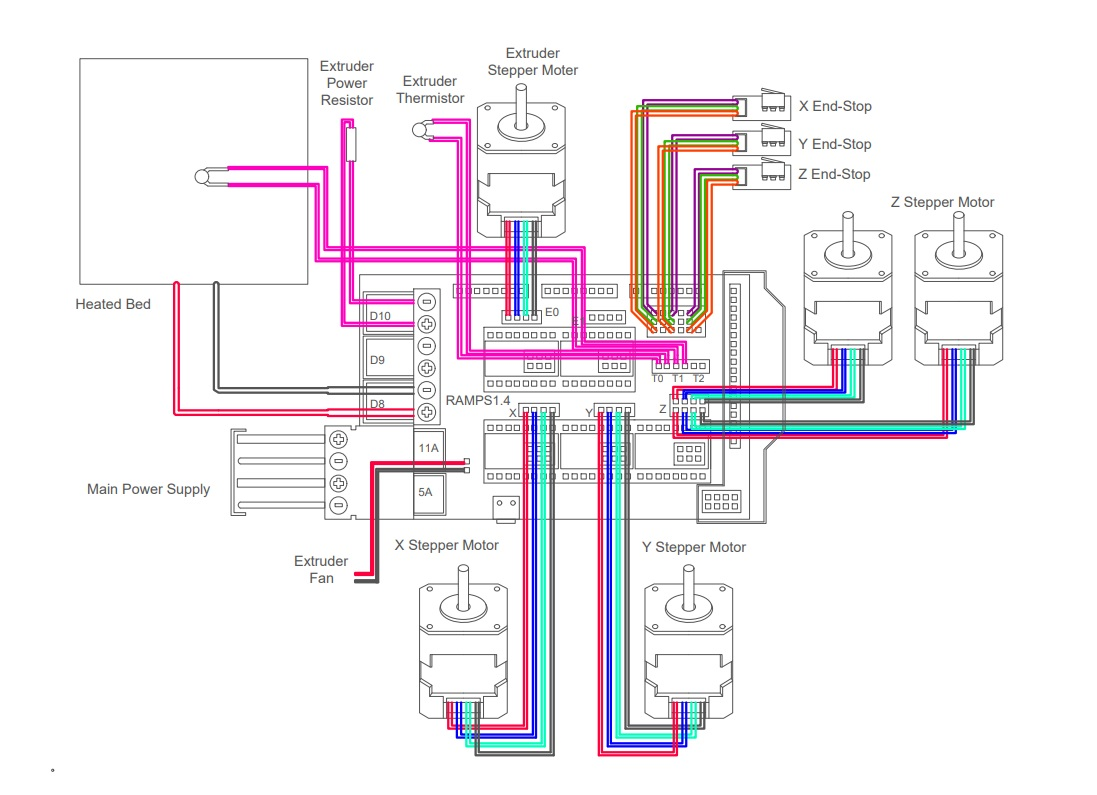
\includegraphics[width=15cm]{接線圖}
\caption{\Large 接線圖}\label{接線圖}
\end{center}
\end{figure}

\section{Arduino Mega 2560}
 Arduino Mega 2560 是基於ATmega2560的主控開發板。Arduino Mega 2560是採用USB接口的核心電路板。它具有54個數位輸入輸出,適合需要大量複雜I/O接口的設計。核心處理器為ATmega2560,有內建Pull-Up電阻在IC內部,不需要在外部電路另外安排Pull-Up電阻,同時具有54路數位輸入/輸出口、16個類比輸入,4個UART接口、1個16MHz晶體振盪器、1個USB連接口、1個電源插孔、1個ICSP接頭以及1個復位按鈕。Arduino Mega 2560也能兼容爲Arduino NUO設計的擴展板。可以自動選擇3中供電方式:外部直流電源通過電源插座供電;電池連接電源連接器的GND和VIN引腳;USB接口直流供電,整合了微控制器以及燒錄功能於一身。\\

\begin{figure}[hbt!]
\begin{center}
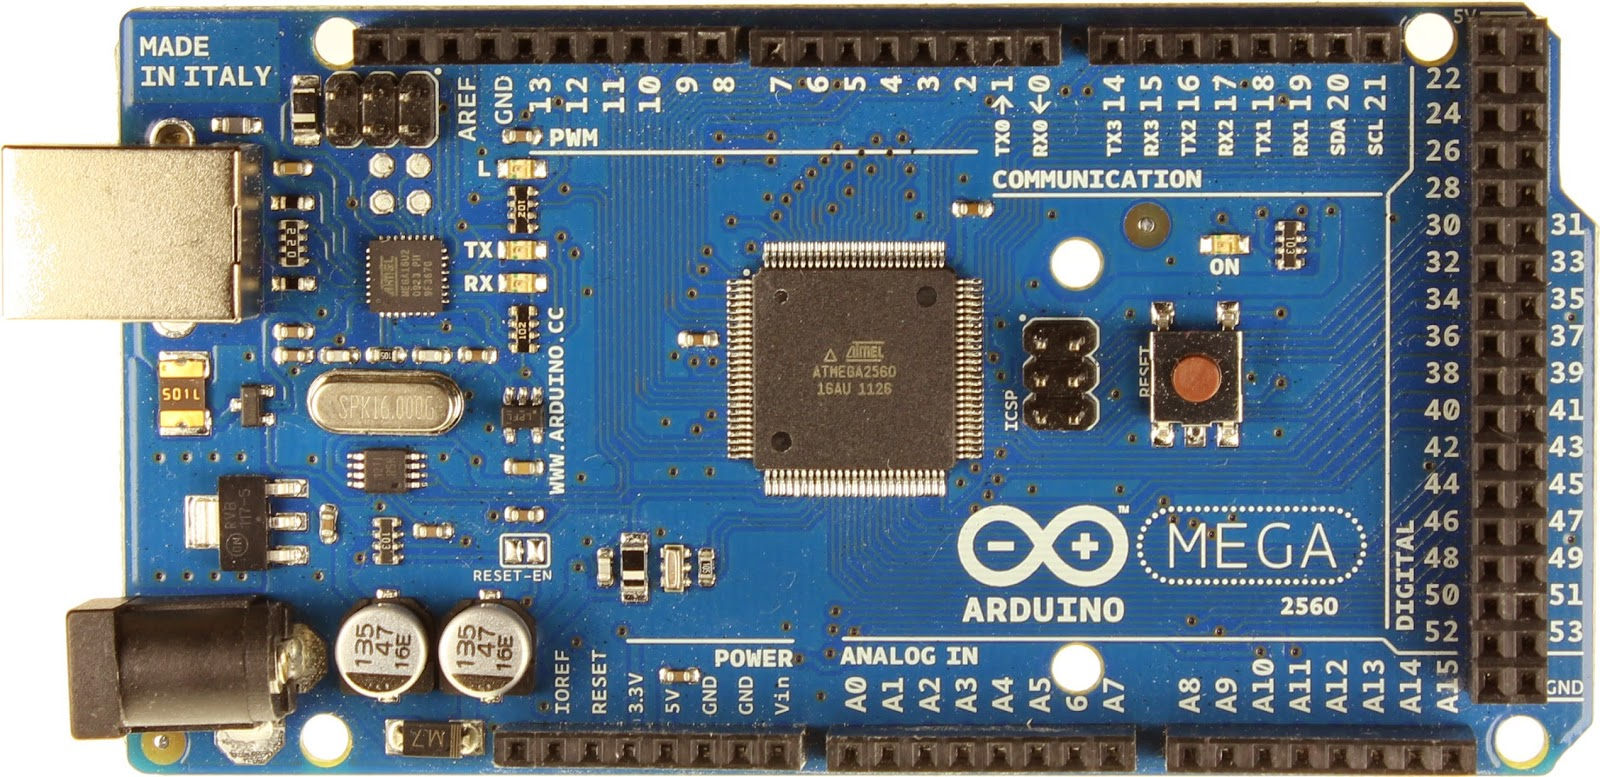
\includegraphics[width=16cm]{ArduinoMega2560}
\caption{\Large Arduino Mega 2560}\label{ArduinoMega2560}
\end{center}
\end{figure}

\newpage

\section{RAMPS 1.4}
 RAMPS 1.4 為RepRap Arduino Mega Pololu Shield的縮寫,主要為設計給步進馬達驅動器的介面電路,1.4為電路版本號碼,目前最新版本為1.7,Arduino Mega 2560可透過RAMPS 1.4介面與控制電路溝通進而達成控制步進馬達以及其他硬體的功能,目前可控制X、Y、Z三軸與最多兩個擠出頭以及兩個散熱風扇。\\
\begin{figure}[hbt!]
\begin{center}
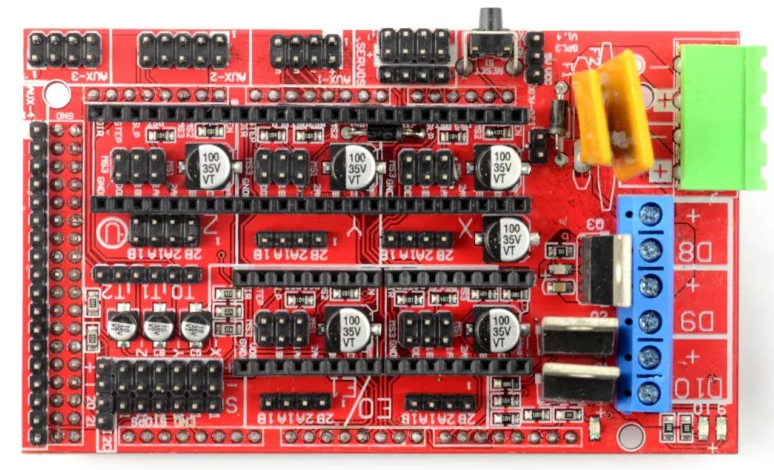
\includegraphics[width=14cm]{Ramps}
\caption{\Large RAMPS 1.4}\label{Ramps}
\end{center}
\end{figure}

\section{其餘元件}

\begin{figure}[hbt!]
\begin{center}
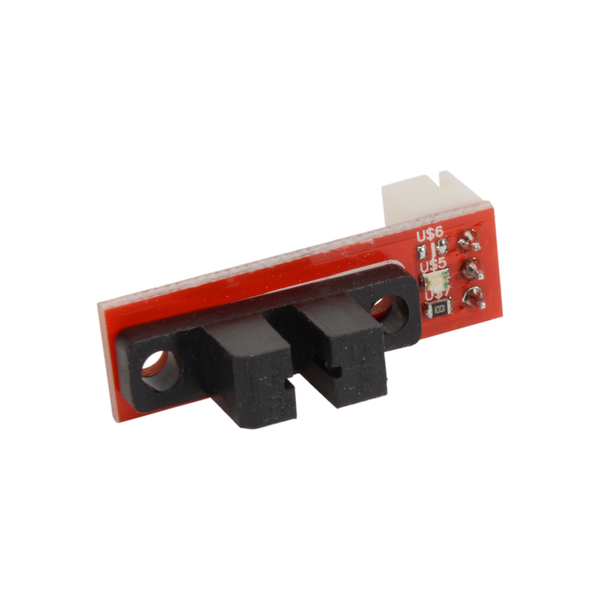
\includegraphics[width=8cm]{endstop}
\caption{\Large 光學限位開關(optical endstop switch)}\label{endstop}
\end{center}
\end{figure}

 光學限位開關的連接需要用到3條線,分別接到RAMPS上的(S)、(-)及(+),這3個腳位。\\

\newpage

\begin{figure}[hbt!]
\begin{center}
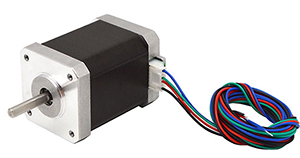
\includegraphics[width=8cm]{NEMA17}
\caption{\Large 步進馬達(Nema 17 Stepper Motors)}\label{NEMA17}
\end{center}
\end{figure}
\begin{figure}[hbt!]
\begin{center}
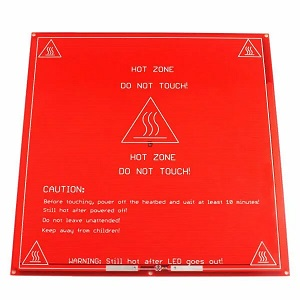
\includegraphics[width=8cm]{Heatbed}
\caption{\Large 加熱床(PCB heatbed)}\label{Heatbed}
\end{center}
\end{figure}
\begin{figure}[hbt!]
\begin{center}
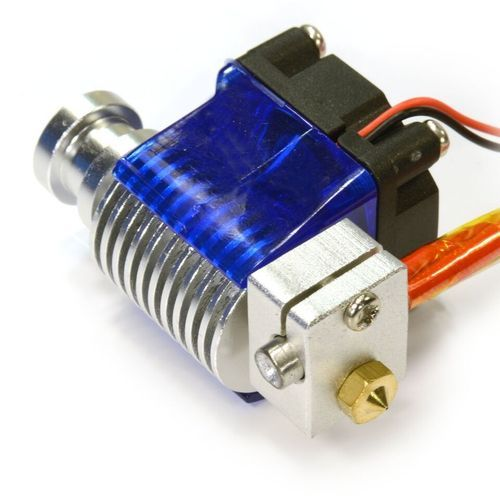
\includegraphics[width=8cm]{Extruder}
\caption{\Large 擠製頭(E3d V6 Hotend)}\label{Extruder}
\end{center}
\end{figure}
\begin{figure}[hbt!]
\begin{center}
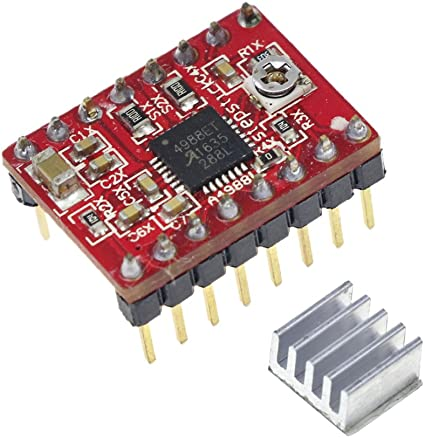
\includegraphics[width=8cm]{A4988}
\caption{\Large A4988 步進馬達驅動器(A4988 Stepper Motor Driver)}\label{A4988}
\end{center}
\end{figure}
\begin{figure}[hbt!]
\begin{center}
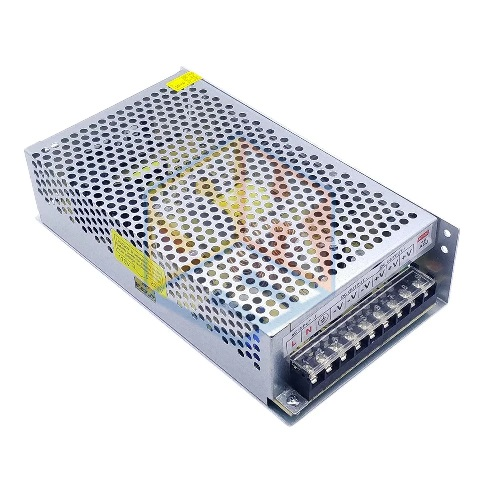
\includegraphics[width=8cm]{Power}
\caption{\Large 電源 12V/20A(Power supply 12V/20A)}\label{Power}
\end{center}
\end{figure}

\newpage 
\chapter{未來研究建議}
本專題已建立2D環境的算法與訓練數據,並將實體系統導入虛擬環境,建立跨平台控制(RemoteAPI)及輔助對打系統,後續可透過建立虛擬環境的訓練程式進行虛擬訓練,完成虛擬訓練後可導入實體機電系統,將對打系統實體化,架設伺服器提供網際介面,提供網際控制、即時觀看對打影像等功能。
\begin{figure}[hbt!]
\begin{center}
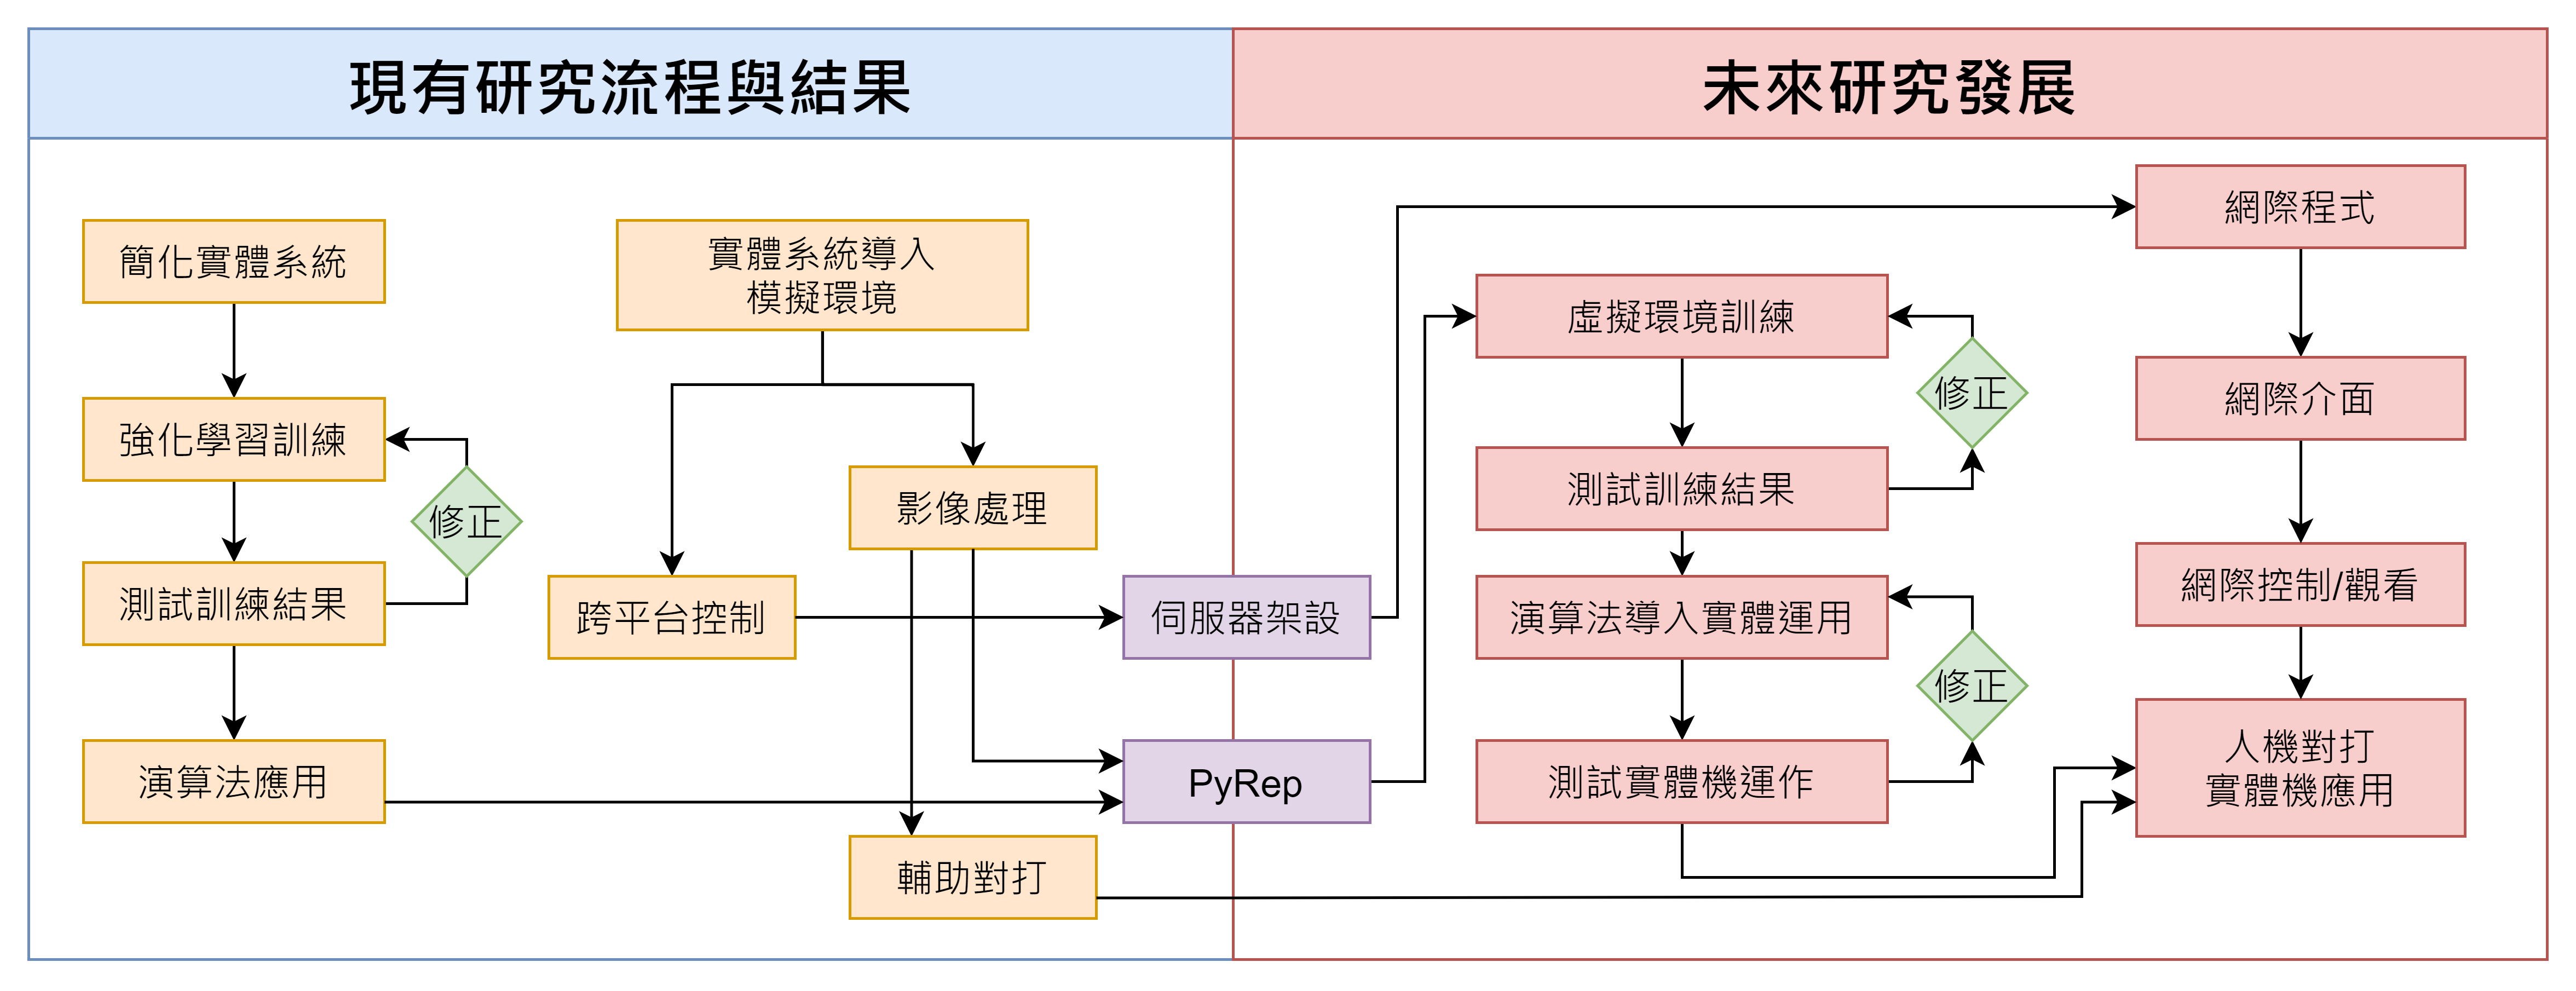
\includegraphics[width=16cm]{現有研究流程與未來展望}
\caption{\Large 現有研究流程與未來展望}
\label{fig.現有研究流程與未來展望}
\end{center}
\end{figure}

\chapter{問題與討論}
\hspace{-1.7em} Q:我們執行sample.py時,python出現了print錯誤。(如:圖8.1)\\
\begin{figure}[hbt!]
\begin{center}
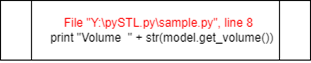
\includegraphics[width=15cm]{print錯誤}
\caption{\Large print錯誤}
\label{print錯誤}
\end{center}
\end{figure}
\newpage
\hspace{-1.4em}A:我們必須把sample.py與pySTL.py裡的全部的print加上括號,才能避免上述狀況的發生。(如:圖8.2)\\

\begin{figure}[hbt!]
\begin{center}
\includegraphics[width=15cm]{print加()}
\caption{\Large print加()}
\label{print加()}
\end{center}
\end{figure}

Q:再次執行sample.py時,pySTL.py出現語法錯誤。(圖.\ref{self.centroid==None語法錯誤})。\\
\begin{figure}[hbt!]
\begin{center}
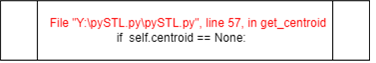
\includegraphics[width=15cm]{self.centroid==None語法錯誤}
\caption{\Large self.centroid==None語法錯誤}
\label{self.centroid==None語法錯誤}
\end{center}
\end{figure}
\qquad \\
A:透過網路的搜尋,找到將==改成is,才可以與None進行比較,所以我們把pySTL裡的line57與line62的==改成is。(如:圖8.4):\\

\begin{figure}[hbt!]
\begin{center}
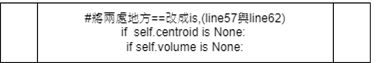
\includegraphics[width=10cm]{將==改成is}
\caption{\Large 將==改成is}
\label{將==改成is}
\end{center}
\end{figure}
%\fontsize{0.001pt}{1pt}\selectfont .\\ %圖片間距勿刪

Q:再次執行sample.py時,pySTL.py出現語法錯誤。(如:圖8.3)。\\
\begin{figure}[hbt!]
\begin{center}
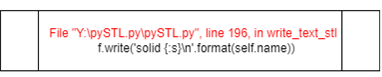
\includegraphics[width=15cm]{self.name錯誤}
\caption{\Large self.name錯誤}
\label{self.name錯誤}
\end{center}
\end{figure}
\qquad \\


A:仔細讀了pySTL裡line196上下的代碼,發現到這段的語法是要開啟ASCII的STL檔案,所以不能使用二進位(wb)的方式來寫入檔案,所以把wb改成w,即可排除上述的錯誤。(如:圖8.4)\\
\begin{figure}[hbt!]
\begin{center}
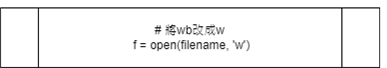
\includegraphics[width=15cm]{將w改成wb}
\caption{\Large 將w改成wb}
\label{將w改成wb}
\end{center}
\end{figure}


Q:再次執行sample.py時,雖然python沒有顯示錯誤,但是寫出的stl檔案格式無法開啟。\\

A:仔細讀了pySTL代碼,發現到line99是使用’rb’來讀取檔案,但是line104裡,沒有使用位元(b)讀取檔案,導致判斷ASCII stl 都會變成binary stl,導致計算ASCII尺寸錯誤無法順利開啟檔案,所以改成b’solid’即可修正問題。(如:圖8.5)\\
\begin{figure}[hbt!]
\begin{center}
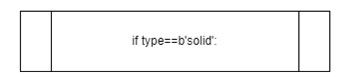
\includegraphics[width=15cm]{type==b'solid'}
\caption{\Large type==b'solid'}
\label{type==b'solid'}
\end{center}
\end{figure}

%=---------------------參考文獻----------------------=%
\addcontentsline{toc}{chapter}{參考文獻} %新增目錄名稱
\newpage
\renewcommand\bibname{參~考~文~獻}
\begin{thebibliography}{99}  % 參考文獻印出之編號最寬為兩個字母寬
\bibitem 1\href{https://create.arduino.cc/projecthub/DesiEngineer/how-to-make-a-big-3d-printer-at-home-using-arduino-4a7b79}{https://create.arduino.cc/projecthub/DesiEngineer/how-to-make-a-big-3d-printer-at-home-using-arduino-4a7b79}
\bibitem 2\href{https://www.coppeliarobotics.com/helpFiles/en/convexDecomposition.htm}{https://www.coppeliarobotics.com/helpFiles/en/convexDecomposition.htm}
\bibitem 3\href{https://web.ntnu.edu.tw/~algo/ConvexHull.html}{https://web.ntnu.edu.tw/~algo/ConvexHull.html}
\bibitem 4\href{https://github.com/neuebot/FIBR3DEmul}{https://github.com/neuebot/FIBR3DEmul}
\bibitem 5\href{https://repositorium.sdum.uminho.pt/bitstream/1822/69730/1/Faria2020_Article_FIBR3DEmulAnOpen-accessSimulat.pdf}{FIBR3DEmulAnOpen-accessSimulat.pdf}
\bibitem 6\href{https://www.ufactory.cc/download-uarm-robot}{https://www.ufactory.cc/download-uarm-robot}
\bibitem 7\href{https://ieeexplore.ieee.org/document/958278}{https://ieeexplore.ieee.org/document/958278}
\bibitem 8\href{https://github.com/proverbialsunrise/pySTL}{https://github.com/proverbialsunrise/pySTL}
\bibitem 9\href{https://zh.m.wikipedia.org/zh-tw/STL}{https://zh.m.wikipedia.org/zh-tw/STL}
\bibitem 0\href{https://stackoverflow.com/questions/3289601/referring-to-the-null-object-in-python}{https://stackoverflow.com/questions/3289601/referring-to-the-null-object-in-python}
\bibitem 1\href{https://hackernoon.com/the-reason-behind-moving-in-the-direction-opposite-to-the-gradient-f9566b95370b}{https://hackernoon.com/the-reason-behind-moving-in-the-direction-opposite-to-the-gradient-f9566b95370b}\label{OGD}
\bibitem 2\href{https://ruder.io/optimizing-gradient-descent/}{https://ruder.io/optimizing-gradient-descent/}
\label{OGD2}
\bibitem 3\href{https://reurl.cc/43XjEL}{https://zh.wikipedia.org/wiki/HSL和HSV色彩空間}
\label{RGBtoHSV}

\bibitem 4\href{https://reurl.cc/gzMm4N}{https://gist.github.com/karpathy/a4166c7fe253700972fcbc77e4ea32c5\# file-pg-pong-py}\label{R.pong1}
\bibitem 5\href{https://reurl.cc/95172Y}{https://github.com/schinger/pongactor-critic/blob/master/pg-pong-ac.py}\label{R.pong1.1}

\bibitem 6\href{https://gist.github.com/etienne87/6803a65653975114e6c6f08bb25e1522}{https://gist.github.com/etienne87/6803a65653975114e6c6f08bb25e1522}\label{R.pong2}

\bibitem 7\href{https://www.ufactory.cc/_files/ugd/896670_cd557a9a80de4e568dafcfb6e27b7240.pdf}{https://www.ufactory.cc/files/ugd/896670cd557a9a80de4e568dafcfb6e27b7240.pdf.}

\bibitem 8\href{https://hdl.handle.net/11296/48s8f5}{https://hdl.handle.net/11296/48s8f5}
\bibitem 9\href{https://zh.wikipedia.org/wiki/%E8%99%9B%E6%93%AC%E5%8C%96}{https://zh.wikipedia.org/wiki/虛擬化}

%\bibitem 10\href
%\bibitem 10\href
%\bibitem 10\href
%
%\bibitem 3\href{https://blog.csdn.net/Csdn_Darry/article/details/107142216}{https://blog.csdn.net/CsdnDarry/article/details/107142216}
\end{thebibliography}
\newpage 
%=---------------附錄-----------------=%
\addcontentsline{toc}{chapter}{附錄} %新增目錄名稱
\begin{appendix}
\renewcommand{\thesection}{\bf 附錄 \Alph{section}}%設定標題名稱
\begin{center}
\fontsize{20pt}{0em}\selectfont\bf 附錄
\end{center}
\section*{LaTeX}
LaTex 為一種程式語言,支援標準庫 (Standard Libraries) 和外部程式庫 (External Libraries),不過與一般程式語言不同的是,它可以直接表述 Tex 排版結構,類似於 PHP 之於 HTML 的概念。但是直接撰寫 LaTex 仍較複雜,因此可以藉由 Markdown 這種輕量的標註式語言先行完成文章,再交由 LaTex 排版。
此專題報告採用編輯軟體為LaTeX,綜合對比Word編輯方法,LaTeX較為精準正確、更改、製作公式等,以便符合規範、製作。
 \begin{table}[htbp] %htbp代表表格浮動位置
			\centering%表格居中
			\caption{文字編輯軟體比較表}%表:標題
			\large%字體大小
			\label{tab_文字編輯軟體比較表:scale}
			\begin{tabular}{|c|c|c|c|c|c|c|}
			\hline
			\diagbox[width=5em]& 相容性 & 直觀性 & 文件排版 & 數學公式 & 微調細部\\
			\hline
			LaTeX 		&$\surd$&		&$\surd$&$\surd$&$\surd$\\
			\hline
			Word	 	&		&$\surd$&		&		&$\surd$\\
			\hline
			
			\end{tabular}
		\end{table}	

\begin{itemize}
\item 特點:
\end{itemize}
\begin{enumerate}
\item 相容性:以Word為例會有版本差異,使用較高版本編輯的文件可能無法以較低的版本開啟,且不同作業系統也有些許差異;相比LaTeX可以利用不同編譯器進行編譯,且為免費軟體也可移植至可攜系統內,可以搭配Github協同編譯。
\item 文件排版:許多規範都會要求使用特定版型,使用文字編譯環境較能準確符合規定之版型,且能夠大範圍的自定義排定所需格式,並能不受之後更改而整體格式變形。
\item 數學公式呈現:LaTex可以直接利用本身多元的模組套件加入、編輯數學公式,在數學推導過程能夠快速的輸入自己需要的內容即可。
\item 細部調整:在大型論文、報告中有多項文字、圖片、表格,需要調整細部時,要在好幾頁中找尋,而LaTeX可以分段章節進行編譯,再進行合併處理大章節。
\end{enumerate}
\begin{figure}[hbt!]
\begin{center}
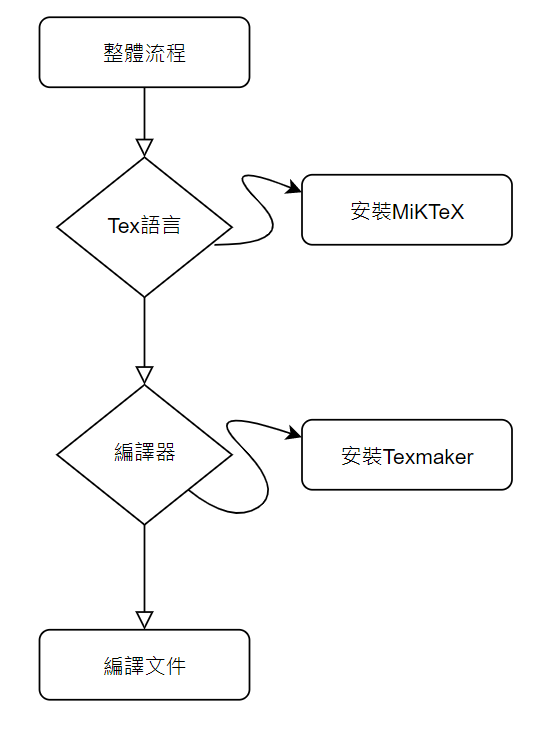
\includegraphics[width=10cm]{編譯流程}
\caption{\Large 編譯流程}
\label{fig.編譯流程}
\end{center}
\end{figure}
\end{appendix}
\newpage
%=-------------作者簡介-----------------=%
    \addcontentsline{toc}{chapter}{作者簡介}
    \begin{center}
	\fontsize{20pt}{0em}\selectfont \bf{作者簡介}\\
	\end{center}	
	{\begin{textblock}{6}(0,0.5)
	\begin{figure}
	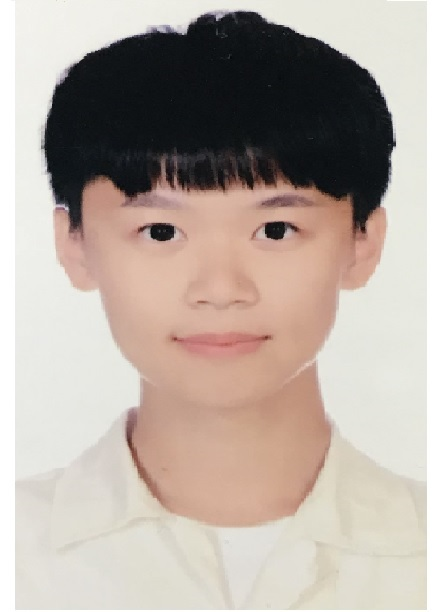
\includegraphics[width=1.25in]{40823116}
	\end{figure}
	\end{textblock}}
	{\renewcommand\baselinestretch{0.99}\selectfont %設定以下行距
	{\begin{textblock}{15}(3.5,0.7)%{寬度}(以左上角為原點之右移量,下移量)
	\noindent\fontsize{14pt}{0em}\selectfont \makebox[4em][s]{姓名}\enspace:\enspace
    \fontsize{14pt}{0em}\selectfont \makebox[4em][s]{江東祐}\\     \hspace*{\fill} \\
    \fontsize{14pt}{0em}\selectfont \makebox[4em][s]{學號}\enspace:\enspace
    \fontsize{14pt}{0em}\selectfont \makebox[4em][s]{40823116} \\ %\makebox為文本盒子
    \hspace*{\fill} \\
    \fontsize{14pt}{0em}\selectfont \makebox[4em][s]{學校}\enspace:\enspace
    \fontsize{14pt}{0em}\selectfont \makebox[9em][s]{國立虎尾科技大學}\\
    \fontsize{14pt}{0em}\selectfont \makebox[5em][s]{\quad}\enspace\enspace
    \fontsize{14pt}{0em}\selectfont \makebox[8em][s]{機械設計工程系}\\
    \hspace*{\fill} \\
    \fontsize{14pt}{0em}\selectfont \makebox[4em][s]{經歷}\enspace:\enspace
    \end{textblock}}}
   % \hspace*{\fill} \\
   \vspace{2em}
	{\begin{textblock}{6}(0,2.3)
	\begin{figure}
	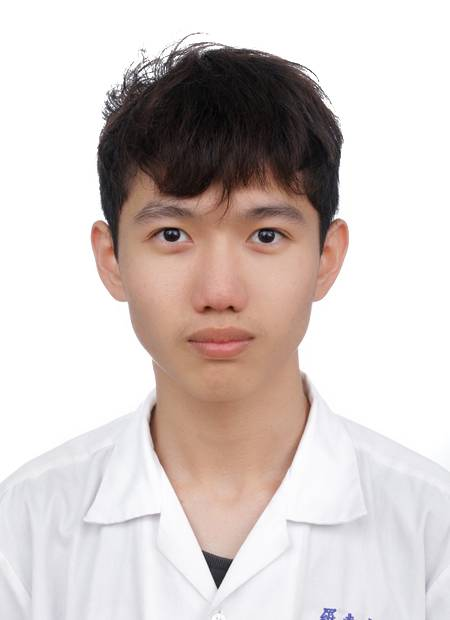
\includegraphics[width=1.15in]{40823131}
    \end{figure}
    \end{textblock}}
    {\renewcommand\baselinestretch{0.99}
    \selectfont %設定以下行距
    {\begin{textblock}{15}(3.5,2.5) %{寬度}(以左上角為原點之右移量,下移量)
\noindent\fontsize{14pt}{0em}\selectfont \makebox[4em][s]{姓名}\enspace:\enspace
\fontsize{14pt}{0em}\selectfont \makebox[4em][s]{江建儒}\\
\hspace*{\fill} \\
\fontsize{14pt}{0em}\selectfont \makebox[4em][s]{學號}\enspace:\enspace
\noindent\fontsize{14pt}{0em}\selectfont \makebox[4em][s]{40823131} \\
\hspace*{\fill} \\
\fontsize{14pt}{0em}\selectfont \makebox[4em][s]{學校}\enspace:\enspace
\fontsize{14pt}{0em}\selectfont \makebox[9em][s]{國立虎尾科技大學}\\
\fontsize{14pt}{0em}\selectfont \makebox[5em][s]{\quad}\enspace\enspace
\fontsize{14pt}{0em}\selectfont \makebox[8em][s]{機械設計工程系}\\
\hspace*{\fill} \\
\fontsize{14pt}{0em}\selectfont \makebox[4em][s]{經歷}\enspace:\enspace
    \end{textblock}}}
    %\hspace*{\fill} \\
    \vspace{2em}
    {\begin{textblock}{6}(0,4.1)
    \begin{figure}
    
\includegraphics[width=1.15in]{40823152} %{}內是圖片文件的相對路徑
    \end{figure}
    \end{textblock}}
    {\renewcommand\baselinestretch{0.99}\selectfont %設定以下行距
    {\begin{textblock}{15}(3.5,4.3) %{寬度}(以左上角為原點之右移量,下移量)
\noindent\fontsize{14pt}{0em}\selectfont \makebox[4em][s]{姓名}\enspace:\enspace%\noindent指定首行不進行縮排
\fontsize{14pt}{0em}\selectfont \makebox[4em][s]{黃暐翰}\\
\hspace*{\fill} \\
\noindent\fontsize{14pt}{0em}\selectfont \makebox[4em][s]{學號}\enspace:\enspace
\noindent\fontsize{14pt}{0em}\selectfont \makebox[4em][s]{40823152} \\ %\makebox為文本盒子
\hspace*{\fill} \\
\noindent\fontsize{14pt}{0em}\selectfont \makebox[4em][s]{學校}\enspace:\enspace
\noindent\fontsize{14pt}{0em}\selectfont \makebox[9em][s]{國立虎尾科技大學}\\
\noindent\fontsize{14pt}{0em}\selectfont \makebox[5em][s]{\quad}\enspace\enspace
\noindent\fontsize{14pt}{0em}\selectfont \makebox[8em][s]{機械設計工程系}\\
\hspace*{\fill} \\
\noindent\fontsize{14pt}{0em}\selectfont \makebox[4em][s]{經歷}\enspace:\enspace
    \end{textblock}}}
   % \hspace*{\fill} \\
   \vspace{2em}
    {\begin{textblock}{6}(0,5.9)
    \begin{figure}
    \includegraphics[width=1.15in]{40823153} %{}內是圖片文件的相對路徑
    \end{figure}
    \end{textblock}}
    {\renewcommand\baselinestretch{0.99}\selectfont %設定以下行距
    {\begin{textblock}{15}(3.5,6.1) %{寬度}(以左上角為原點之右移量,下移量)
\noindent\noindent\fontsize{14pt}{0em}\selectfont \makebox[4em][s]{姓名}\enspace:\enspace
\noindent\fontsize{14pt}{0em}\selectfont \makebox[4em][s]{蕭日傑}\\ \hspace*{\fill} \\
\noindent\fontsize{14pt}{0em}\selectfont \makebox[4em][s]{學號}\enspace:\enspace
\noindent\fontsize{14pt}{0em}\selectfont \makebox[4em][s]{40823153} \\ \hspace*{\fill} \\
\noindent\fontsize{14pt}{0em}\selectfont \makebox[4em][s]{學校}\enspace:\enspace
\noindent\fontsize{14pt}{0em}\selectfont \makebox[9em][s]{國立虎尾科技大學}\\
\noindent\fontsize{14pt}{0em}\selectfont \makebox[5em][s]{\quad}\enspace\enspace
\noindent\fontsize{14pt}{0em}\selectfont \makebox[8em][s]{機械設計工程系}\\
\hspace*{\fill} \\
\noindent\fontsize{14pt}{0em}\selectfont \makebox[4em][s]{經歷}\enspace:\enspace
    \end{textblock}}}
    %\hspace*{\fill} \\
\newpage
%=----------------書背----------------------=%
\pagestyle{empty}%設定沒有頁眉和頁腳
\begin{center}
\fontsize{0.001pt}{1pt}\selectfont .\\
\vspace{4em}
\fontsize{30pt}{30pt}\selectfont 【13】 \\
\fontsize{15pt}{15pt}\selectfont
\vspace{0.5em}
分\\
類\\
編\\
號\\
\vspace{0.5em}
\hspace{-0.5em}:\\
\vspace{0.5em}
\rotatebox[origin=cc]{270}{\sectionef\LARGE \textbf{111-4-APP-3004-1}}\\ %旋轉
\vspace{0.5em}
3D\\
列\\
印\\
模\\
擬\\
在\\
機\\
械\\
手\\
臂\\
設\\
計\\
上\\
的\\
應\\
用\\
\vspace{2em}
一\\
一\\
一\\
級\\

\end{center}
%\newpage
%\begin{landscape}  %橫式環境
%\begin{center}
%\fontsize{0.001pt}{1pt}\selectfont .
%\vspace{70mm}
%\rotatebox[origin=cc]{90}{\LARGE 【14】}\rotatebox[origin=cc]%{180}{\LARGE 1-2-APP-8765} %旋轉
%\end{center}
%\end{landscape}
\end{document}
